% !TeX spellcheck = de_DE 
\chapter{Implementierung}
\label{sec:imp}
In meiner Abschlussarbeit präsentiere ich die praktische Lösung für das PSE-Labor der Beuth Hochschule für Technik Berlin. Die gesamte Aufgabe lässt sich in drei Bestandteile unterteilen: Register-Client, Server und Display-Client. Erstens wird Register-Client implementiert, damit wird RFID Leser am Raspberry Pi Mikrocomputer angeschlossen, alle Treiber installiert und auf Python Programmierung Sprache die Software geschrieben, die die ständige Überwachung des empfangenden von RFID Leser Daten zulässt und die Verbindung mit dem Server zulässt. Falls die empfangene Daten korrekt sind, d.h.  eine richtige MIFARE Studentenkarte oder einen richtigen RFID-Transponder abgelesen wurde, schickt die Software die abgelesene Daten zum Server ab. Der Server ist der zweite Bestandteil der Abschlussarbeit und wird mit Hilfe Django Framework, Django Finite State Machine auf Python Programming Sprache implementiert. Server enthält die Datenbank mit die Datensätzen über die alle im PSE-Labor vorhandenen ausleihenden Boards, die zum Modul im laufenden Semester registrierten Studenten und  geschehenen Ausleihe/Rückgabe-Vorgänge. Es wird von Server überprüft, ob eine von Register-Client abgelesene Studentenkarte einem zugelassenen für die Ausleihe Student gehört und die entsprechenden Information auf Display-Client geschickt. Es wird auch von Server bestätigt, ob für die Ausleihe/Rückgabe neben dem RFID-Leser gehaltenen Raspi Board dem Student ausgeliehen/vom Student zurückgegeben werden darf. Darauf aufbauend, wird der dritte Teil namens ein Display-Client als dynamische HTML-Seite realisiert, die eine Verbindung zum Server Mithilfe des HTTP-Protokolls und eingebauten im Browser Kommunikationsmittel die asynchrone Nachrichten zu schicken, bereitstellt. Für die dynamische Aktualisierung des Inhalts der Webseite und einen Zugang zum asynchronen HTTP-Client wird jQuery benutzt.
\section{Register-Client}
\label{sec:register_client}
Das folgende Kapitel beschäftigt sich mit der Implementierung des Register-Client auf Raspberry Pi Board mit angeschlossenen RFID-Leser. Dieser Teil der verteilte System lässt sich wie folgendes unterteilen. Zuerst wurde das Betriebssystem Raspbian auf Board zum Leben gebracht und dann die alle notwendigen für RFID-Leser Treiber installiert. Nach dem der RFID-Leser funktionieren angefangen und die Daten von RFID-Transponder abgelesen hat, wurde die nächste Herausforderungen gelöst: die Struktur die zu empfangenen Daten wurde verstanden, richtig bearbeitet, eine JSON-Datei erstellt und durch die HTTP-Protokoll dem Server geliefert. 

\subsection{Installation des Betriebssystem}
\label{sec:register_client:raspbian}
Der vorhandene für die Abschlussarbeit Raspberry Pi 3 Model B+ wurde nicht als Starter Kit mir übergeben, dann wurde es zusätzlich benötigt \cite[pp. 21-22]{gareth:raspi}: 
\begin{itemize}
	\item \textbf{USB-Netzteil} mit einer Nennleistung von 2,5 A (2,5 A) oder 12,5 Watt (12,5 W) und einem Micro-USB-Anschluss. 
	\item \textbf{microSD-Karte}, die als permanenter Speicher des Raspberry Pi dient; Alle von Benutzer erstellten Dateien und die installierte Software sowie das Betriebssystem selbst werden auf der microSD-Karte gespeichert.
	\item \textbf{USB-Tastatur und -Maus}, mit denen den Raspberry Pi gesteuert werden kann. Fast jede kabelgebundene oder kabellose Tastatur und Maus mit USB-Anschluss funktioniert mit dem Raspberry Pi.
	\item \textbf{Das HDMI-Kabel}, das Ton und Bilder vom Raspberry Pi auf Fernseher oder Monitor überträgt. Sie müssen nicht viel Geld für ein HDMI-Kabel ausgeben. 
\end{itemize}

Die Arbeit mit einem RaspberryPi setzt ein paar Anfangsinvestitionen voraus, die auch von den angestrebten Aufgaben und Projekten abhängen. Zuerst gäbe es die Möglichkeiten, dass der gekaufte Raspberry Pi Board bereits ein Betriebssystem darauf installiert hätte. Aber es war nicht der Fall von vorhandenen im PSE-Labor Board. Um ein Betriebssystem auf diesen Raspberry Pi zu bringen, muss eine SD-Karte mit einem Betriebssystem-Image "geflasht" werden. Dafür zunächst wurde die Distribution von der Website Raspbian.org herunterladen und die MicroSD-Karte in den Kartenleser eines vorhandenen im PSE-Labor PC eingelegt. Anschließend wurde mit dem Macintosh Disk Utility-Dienstprogramm das heruntergeladene und entpackte Betriebssystem für den RaspberryPi auf eine Speicherkarte geschrieben. Dann ist die Karte in Raspberry Pi einzulegen. Der Raspi ist damit betriebsbereit und muss für die zukünftigen Anwendungen noch konfiguriert werden. Wenn der Pi zum ersten Mal eingeschaltet wird, wird viel Text auf dem Bildschirm angezeigt. Diese werden als Startmeldungen bezeichnet. Wenn Raspbian zum ersten Mal gestartet wurde, kann es ein oder zwei Minuten dauern, um die Nutzung des freien Speicherplatzes auf der microSD-Karte optimal anzupassen. Beim nächsten Start geht es schneller. Schließlich ist kurz ein Fenster mit dem Raspberry Pi-Logo zu sehen, dann wird Terminal Fenster angezeigt, in dem es einloggt werden muss. Zum ersten Einloggen wird den Standardbenutzername "pi" und das Standardkennwort  "raspberry" verwendet. Um Register-Client vor sowohl Online-Bedrohungen als auch von Missbrauch im Labor zu schützen, wurde das Standardkennwort sofort geändert. Der nächste Schritt ist Raspbian bis zur Version "Raspbian mit dem Raspberry Pi Desktop" zu aktualisieren, damit die grafische Benutzeroberfläche und Chromium Browser zu Verfügung stehen können. Dies kann mit dem Terminalbefehl gemacht werden:
\begin{lstlisting}[caption={[Terminalbefehl für die Installation der GUI] },captionpos=b]
sudo apt-get install lxde-core xserver-xorg xinit
\end{lstlisting}
Dann ist der Raspberry Pi erneut zu laden. Nachdem Raspberry Pi-Logo wieder angezeigt wurde, wäre der Raspbian-Desktop zu sehen. Somit gilt Betriebssystem als vollständig installiert und kann benutzt werden. Das war aber nicht der Fall mit dem vorhandenen Hardware, da es plötzlich eine Boot-Schleife vorkam, nachdem der Mikrocomputer eingeschaltet wurde und der Startvorgang nicht abgeschlossen werden konnte. Anstatt das zum Benutzung bereiteten Betriebssystem mit der grafische Benutzeroberfläche zu sehen,  wird eine Schleife erzeugt, in der die Startvorgang kontinuierlich und wiederholt ausgeführt wurde und somit eine Nutzung der Mikrocomputers unmöglich ist. Nach den mehreren Recherchen wurde es vermutet, dass es durch eine unzureichende Stromversorgung verursacht werden könnte. Es wurde aber zuerst nicht versucht, einen USB-Netzteil zu wechseln, da die anderen USB-Netzteil man durch PSE-Labor bestellen und eine Zeit abwarten muss. Jedoch wurde eine erzeugte Boot-Schleife mit einem anderen Terminalbefehl erfolgreich gelöst:
\begin{lstlisting}[caption={[Boot-Schleife beim Start des der Desktops] },captionpos=b]
sudo apt-get install --reinstall pcmanfm
\end{lstlisting}
Bei der Arbeit mit dem Mikrocomputer tritt jedoch später ein Problem mit der Stromversorgung auf. Der Fall kann im entsprechenden Kapitel \ref{sec:register_client:voltage_issue} nachgelesen werden.


\subsection{Installation der Treibers für RFID-Leser}
\label{sec:register_client:install_rfid}
Im weiteren Verlauf der Arbeit wird den RFID Leser/Schreiber ACR122U erfolgreich angefahren, der auf der Basis der 13,56 MHz kontaktlosen (RFID ) Technologie entwickelt wurde. Der ACR122U USB Kartenleser unterstützt nicht nur Mifare ® Technologien, sondern auch alle vier Typen von NFC -Tags. Diese Anforderung ist für vorliegende Abschlussarbeit wichtig, da Studierenden-Ausweise der Beuth Hochschule mit dieser Technologie gelesen werden können. Obwohl Raspbian mit einer Reihe von Software vorinstalliert ist, wird es aber zusätzlich benötigt, die Treiber für RFID-Leser zu installieren. Es sollte an dieser Stelle auch noch angemerkt werden, dass am Anfang der Entwicklungsprozess ein anderen RFID-Leser angeschlossen wurde als der, den in der Abschlussarbeit zu beschreiben und zu beobachten ist. Zuerst wurde die Treiber für Reiner SCT CyberJack RFID Basis \cite{website:4} installiert. Die Schritte sollten in der Abschlussarbeit nicht unerwähnt bleiben, da die damals für den ersten RFID-Leser installierte Treiber und Daemons (Appendix \ref{sec:appendix:daemon}) wurden endlich für den zweiten RFID-Leser benutzt, mit dem die Entwicklung der Aufgabe abgeschlossen wurde. Der Grund für die Hardwareaustausch ist die festgestellte Tatsache, dass Reiner SCT CyberJack RFID Leser die Studentenkarten nicht ablesen konnte. Obwohl in der Spezifikation es steht, dass die Reiner RFID-Leser kontaktlose RFID Chipkarten wie eID mit dem neuen Personalausweis (nPA), GeldKarte oder eTicketing unterstützt, wurde es unmöglich mit den MIFARE-Transponder 13,561 MHz Funkbereich ins Spiel zu bringen. Die Studierenden-Ausweise der Beuth sollten mit dieser Technologie gelesen werden und somit ist diese Anforderung für die vorliegende Abschlussarbeit wichtig. 

Um RFID-Leser anzuschließen, muss man den Leser über USB mit einem Raspberry Pi verbunden. Der Typ des RFID-Lesegeräts, der für die vorliegende Abschlussarbeit verwendet wird, ist ein ACR122U-A9 von Advanced Card Systems\cite{website:7}, den auf der Abbildung\ref{fig:rfid_hard} zu sehen. Zuerst müssen wir die Paketlisten aktualisieren und einige Pakete herunterladen und installieren \cite{website:6}: Die folgenden Abhängigkeiten werden benötigt im System mit dem Befehl "sudo apt-get install" zu installieren: $libusb-dev, libpcsclite-dev, libpcsclite1, libccid, pcscd, pcsc-tools, libpcsc-perl, libusb-1.0-0-dev, libtool, libssl-dev$.\\
\begin{wrapfigure}{l}{0.45\textwidth}
	\fbox{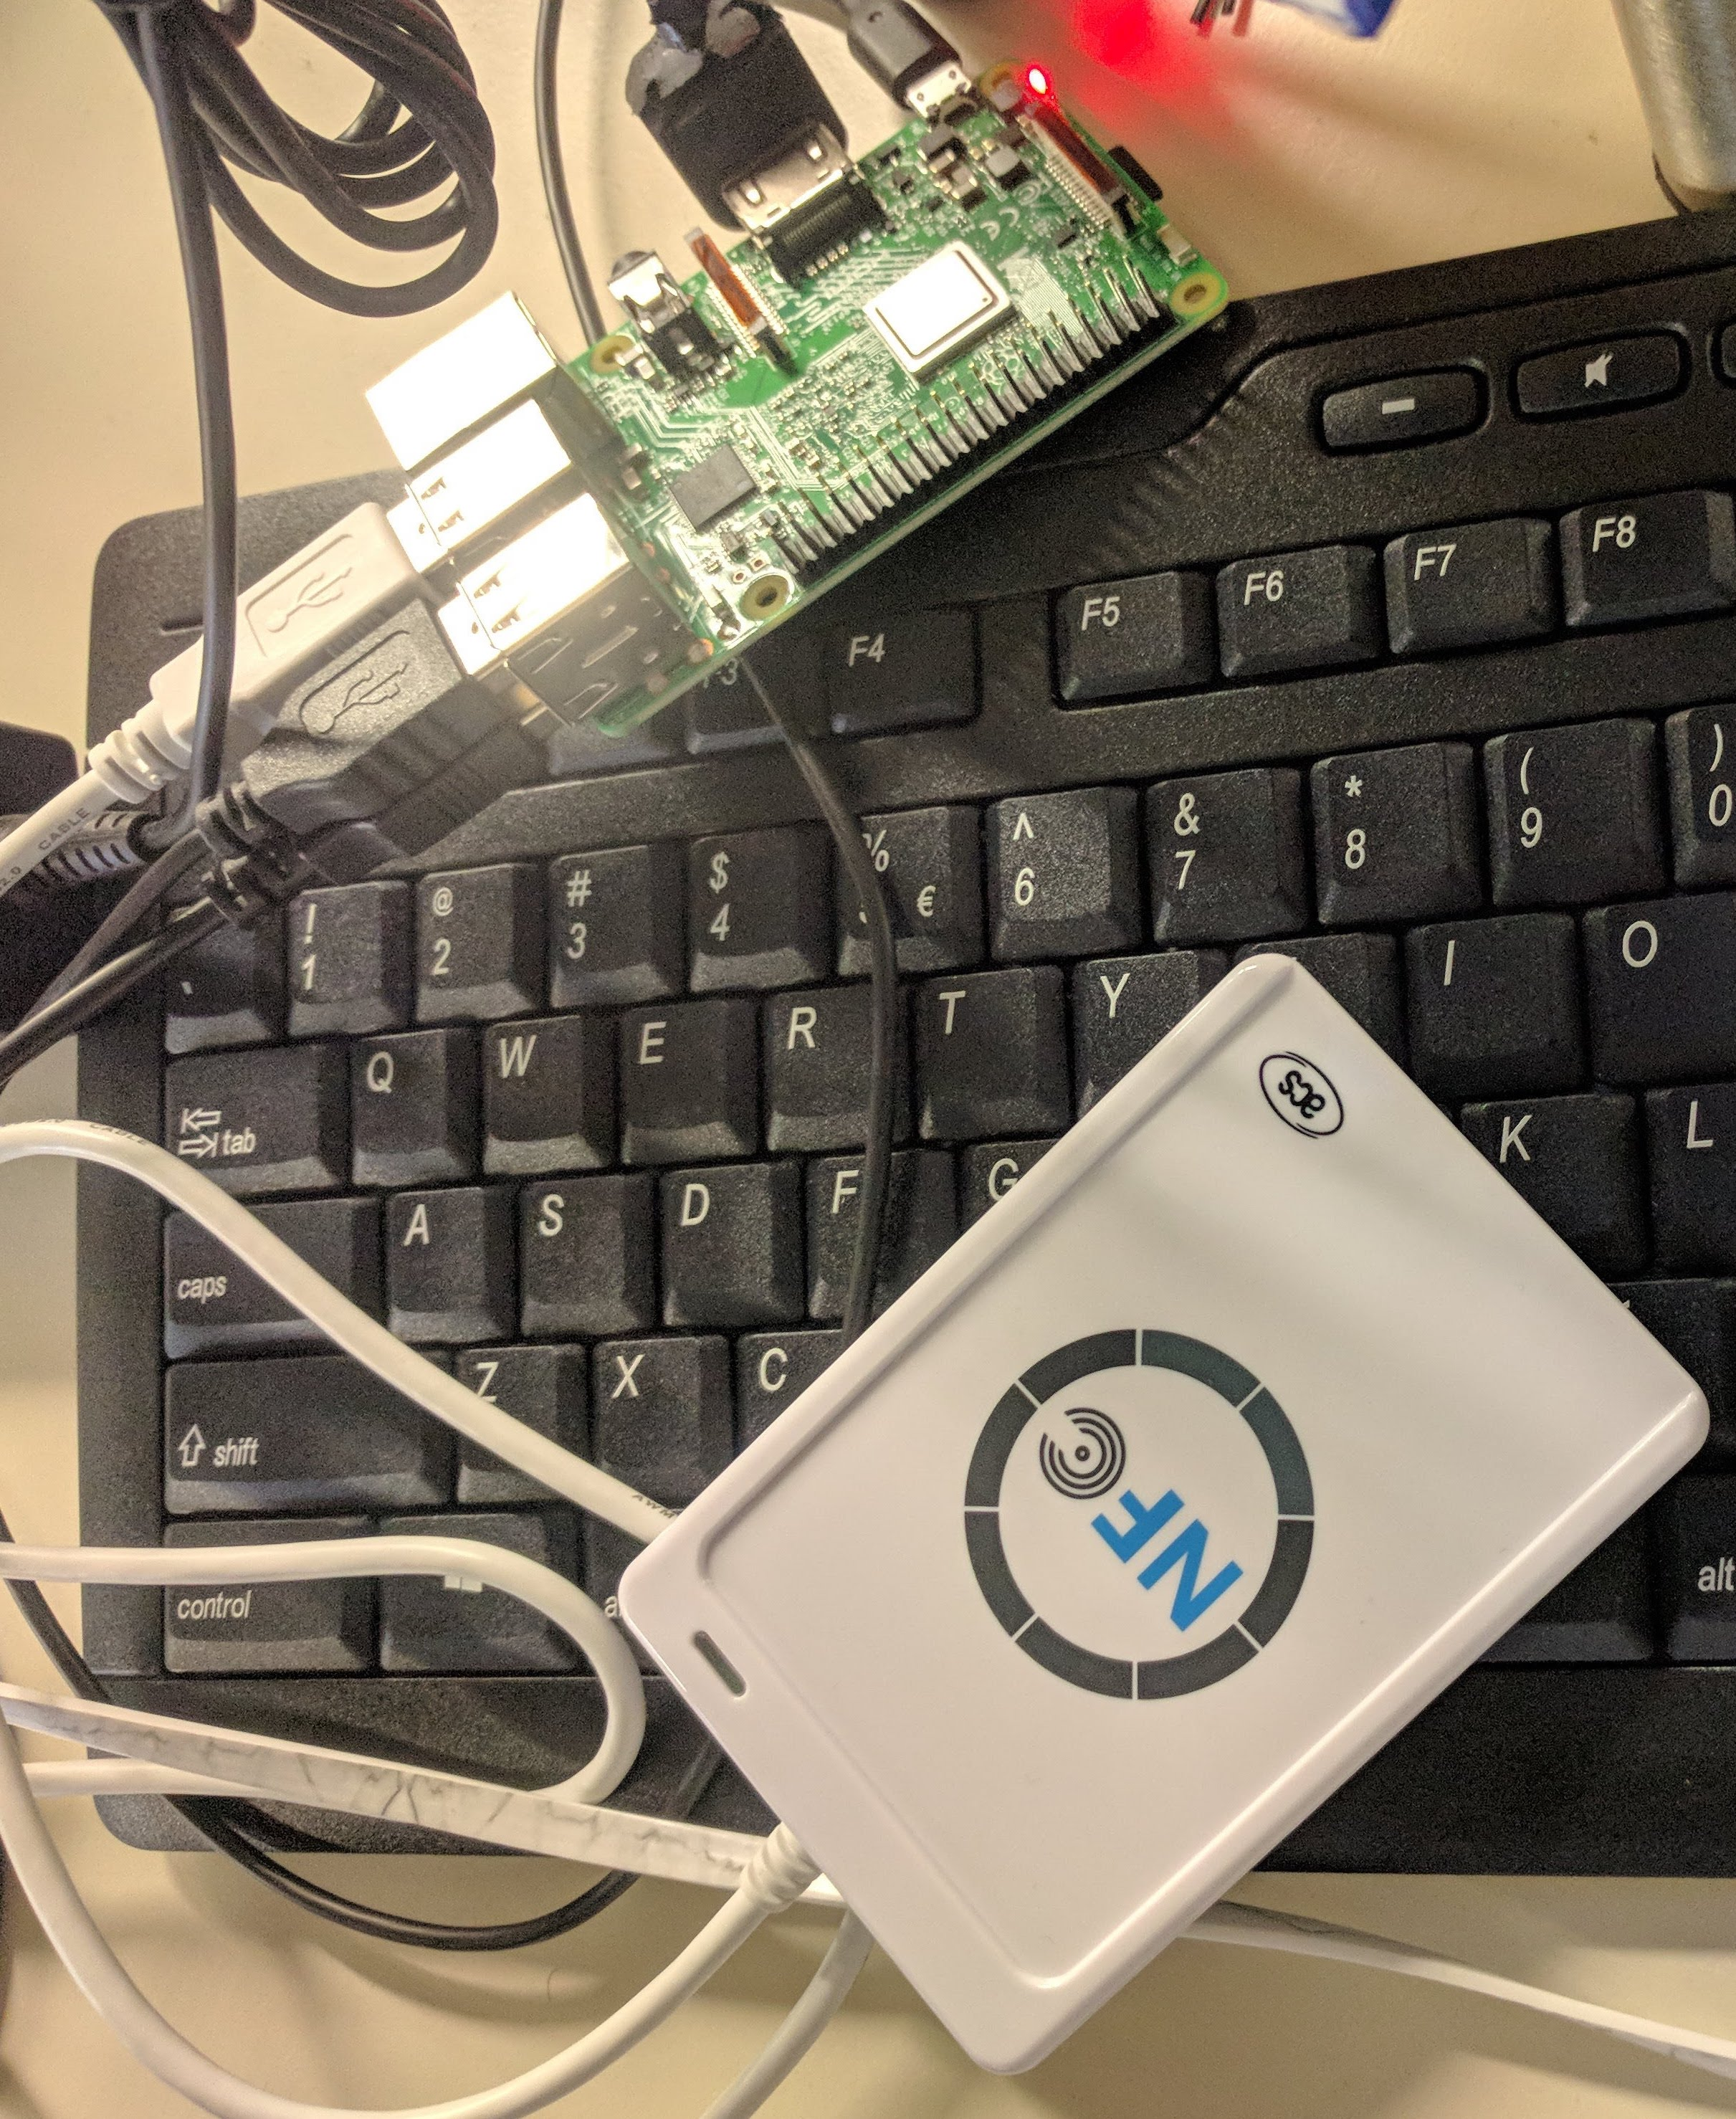
\includegraphics[width=0.42\textwidth]{gfx/rfid_hard.jpg}}
	\caption{ACR122U-A9 von Advanced Card Systems und Raspbery Pi}
	\label{fig:rfid_hard}
\end{wrapfigure}
PC/SC ist ein Standard für die Schnittstelle von Computern mit Smartcards, der auf den meisten Betriebssystemen, einschließlich Windows und Linux, verfügbar ist. PC/SC-Kopplungsgeräte benötigen einen Treiber, mit dem Anwendungen die Karte einfach erreichen können. Da PC/SC für Smartcards entwickelt wurde - und in einer Zeit, in der Smartcards nur Kontaktkarten waren funktioniert es auch mit den kontaktlosen Karten, falls RFID-Leser es unterstützt. Das Daemon-Programm für pcsc-lite namens pcscd koordiniert die Kommunikation mit Smartcard-Lesegeräten und Smartcards sowie kryptografischen Tokens, die mit dem System verbunden sind. Normalerweise wird pcscd beim Booten von /etc/init.d/pcscd gestartet. Damit können Anwendungen auf Smartcards und Lesegeräte zugreifen, ohne die Details der Karte oder des Lesegeräts zu kennen. Das Laden von Treibern für Kartenleser wird von pcscd koordiniert. Der Zweck von pcsc-lite besteht darin, eine kompatible API (Winscard) für die Migration von Windows-basierten PC / SC-Anwendungen auf Unix bereitzustellen \cite{website:5}. Die allgemeinen Zugriff auf USB-Geräte bietet eine C-Bibliothek namens libusb.  Sie soll von Entwicklern verwendet werden, um die Produktion von Anwendungen zu erleichtern, die mit USB-Hardware kommunizieren. Es ist portabel, da mit einer einzigen plattformübergreifenden API auf USB-Geräte unter Linux, MacOS, Windows usw. zugegriffen werden kann. Sie wird im Benutzermodus ausgeführt und somit für die Kommunikation der Anwendung mit einem Gerät keine besonderen Berechtigungen oder Erhöhungen erforderlich sind \cite{website:88}.

Dann laden wir die Open-Source-Bibliothek libnfc für Near Field Communication (NFC) herunter, extrahieren, konfigurieren und installieren es. Nach der erfolgreichen Installation kann den verbindenden über USB RFID-Leser mithilfe des Tools lsusb angesehen werden: es wird VendorId und ProductID angezeigt. Es ist auch notwendig die abgelesene VendorId und ProductID in der entsprechenden XML-Datei. Die Datei auf der MicroSD-Karte ist zu finden :
\begin{lstlisting}[caption={[XML-Datei für VendorId und ProductID] },captionpos=b]
/usr/lib/pcsc/drivers/ifd-ccid.bundle/Contents/info.plist
\end{lstlisting}

\subsection{Spannungsproblem und Lösung}
\label{sec:register_client:voltage_issue}
Nachdem der RFID-Leser angeschlossen wurde, tritt es ein weiteres Problem, das die freie Benutzung der Raspberry Pi unmöglich macht. Es wird unabhängig von der Zeit und vorherigen Geschehen eine Fehlermeldung "under voltage detected (0x000050000000)". Es wird zuerst versucht die kabellose USB-Tastatur und -Maus abzuschalten. USB eine aktive Abfrage seine Ports (Polling) benötigt, was bedeutet, dass die Anzahl der für andere Aufgaben verfügbaren CPU Zyklen geringer ist. Dies kann dazu führen, dass die CPU-Frequenz ansteigt, wodurch der Stromverbrauch höher wäre. Es wurde festgestellt, dass mit unverbundenen USB-Tastatur und -Maus die Fehlermeldung trotzt vorkommt. Nur wenn der RFID-Leser angeschaltet wurde, kam es keine neue Fehlermeldung. Dann es wurde geprüft, ob ausgewählten RFID-Leser mit dem vorhandenen Mikrocomputer überhaupt kompatibel ist und nach der Lösung gesucht, mit der die zukünftige Entwicklung weiterlaufen kann.    

Anfänglich wurde als Spannungsversorgungsteil ein USB-Netzteil von einem modernem bei Autorin der Abschlussarbeit vorhandenen zu Hause Smartphone benutzt. Das offizielle Raspberry Pi-Netzteil ist die empfohlene in der Dokumentation Wahl, jedoch wurde zuerst mit dem Mikrocomputer nicht gekauft. Ein leistungsfähiger USB-Netzteil könnte den schnell wechselnden Strombedarf des Raspberry Pi bewältigen. Nach der Besprechung des Problems mit den PSE-Labor Mitarbeiter wurde ein Samsung USB-Netzteil gegen einen Anker USB-Netzteil ausgetauscht und festgestellt, dass das Spannungsproblem mit den verbundenen sowohl USB-Tastatur und -Maus als auch RFID-Leser während des Ablesevorgangs nicht wieder erscheint. 

\subsection{Python Programmierung des RFID-Lesers}
\label{sec:register_client:smart}
Nachdem es gelingt mir, die Hardware angefahren und die ersten Studentenkarte so abzulesen, dass es ein Schallton von RFID-Leser erzeugt wurde, sollte eine weitere Aufgabe gelöst werden: die Daten von RFID-Tag auf einem auszuleihenden Raspi Board von Studentenkarte unterscheiden zu können. Es sollte ausgeschlossen werden, dass ein Ausleihe-/Rückgabevorgang angefangen wird, falls eine falsche Studentenkarte (z.B. mit einer BVG Jahresfahrkarte) am RFID-Leser präsentiert wird. Als es im Kapitel \ref{sec:theorie:mifare} erklärt wurde, sind die neuen Campus Karte der Beuth Hoschule für Technik Berlin mit den die MIFARE-Transponder hergestellt. Für die Programmierung des RFID-Lesers wird Smartcard-Schnittstelle benutzt, deren Installierung geschah zusammen mit pyscard und im Kapitel \ref{sec:register_client:install_rfid} geschrieben. Diese Schnittstelle steht für den Entwickler für die Arbeit mit Smartcards und NFC-Geräten zur Verfügung, sie wird in Form mehrerer Systemdienste implementiert und ihr Schnittstellenteil ist das PC/SC-Framework. PC/SC steht für Personal Computer/Smart Card.

Es steht mehreren Möglichkeiten für die Entwicklung eine Sprache zu wählen: die Funktionen der Smartcard-Schnittstelle können mit Python, C/C++ und Java Sprache verwendet werden. Die Programmierung des Register-Clients wird auf Python Sprache gemacht, dieselbe Sprache wird für Server während der Arbeit mit Django Framework benutzt. Die Entwicklung mit dem Importieren der PCSC-Header-Dateien beginnt. 
\begin{lstlisting}[caption={[Importieren der PCSC-Header-Dateien] },captionpos=b]
from smartcard.System import readers
from smartcard.ATR import ATR
from smartcard.CardMonitoring import CardMonitor, CardObserver
from smartcard.CardRequest import CardRequest
\end{lstlisting}
Wann eine RFID-Leser über USB angeschlossen wird, kann es eine Verbindung zur PC/ SC-Bibliothek hergestellt und eine Liste der verfügbaren Terminals abgerufen werden. Alle API-Funktionen geben einen Statuscode zurück. Wenn die Funktion erfolgreich ist, wird die Konstante  $SCARD\_S\_SUCCESS$  zurückgegeben. Alle anderen Daten werden über Funktionsargumente zurückgegeben, in denen die Adresse der gewünschten Variablen übergeben wird. Die Verbindung (Initialisierung) erfolgt über die Funktion $SCardEstablishContext()$ \cite[p. 101]{chirico:smart_card}. Die Adresse der Variablen $sc\_context$ vom Typ $SCARDCONTEXT$ wird an sie übergeben. Als Nächstes müssen Sie eine Liste der Terminals abrufen. Dies erfolgt über die Funktion $SCardListReaders()$. Dann muss die Liste der angeschlossenen Lesers erhalten und gelesen. Es ist eine Reihe von Zeichenfolgen, die durch ein Nullbyte getrennt sind. Dies ist ein Windows-Format zur Darstellung von Zeichenfolgenlisten und wird üblicherweise als Zeichenfolge mit doppelter Nullterminierung bezeichnet. Durch Aufrufen der Funktion $SCardListReaders()$ erhalten wir eine Liste aller Namen \cite[p. 102]{chirico:smart_card}. Da in Abschlussarbeit es ist vorgesehen, dass nur ein RFID-Leser über USB am Register-Client angeschlossen werden darf, wird nur ein Name nach der Funktionsausruf zurückgegeben:
\begin{lstlisting}
Found readers: ['ACS ACR122U']
\end{lstlisting}

\begin{wrapfigure}{l}{0.45\textwidth}
	\fbox{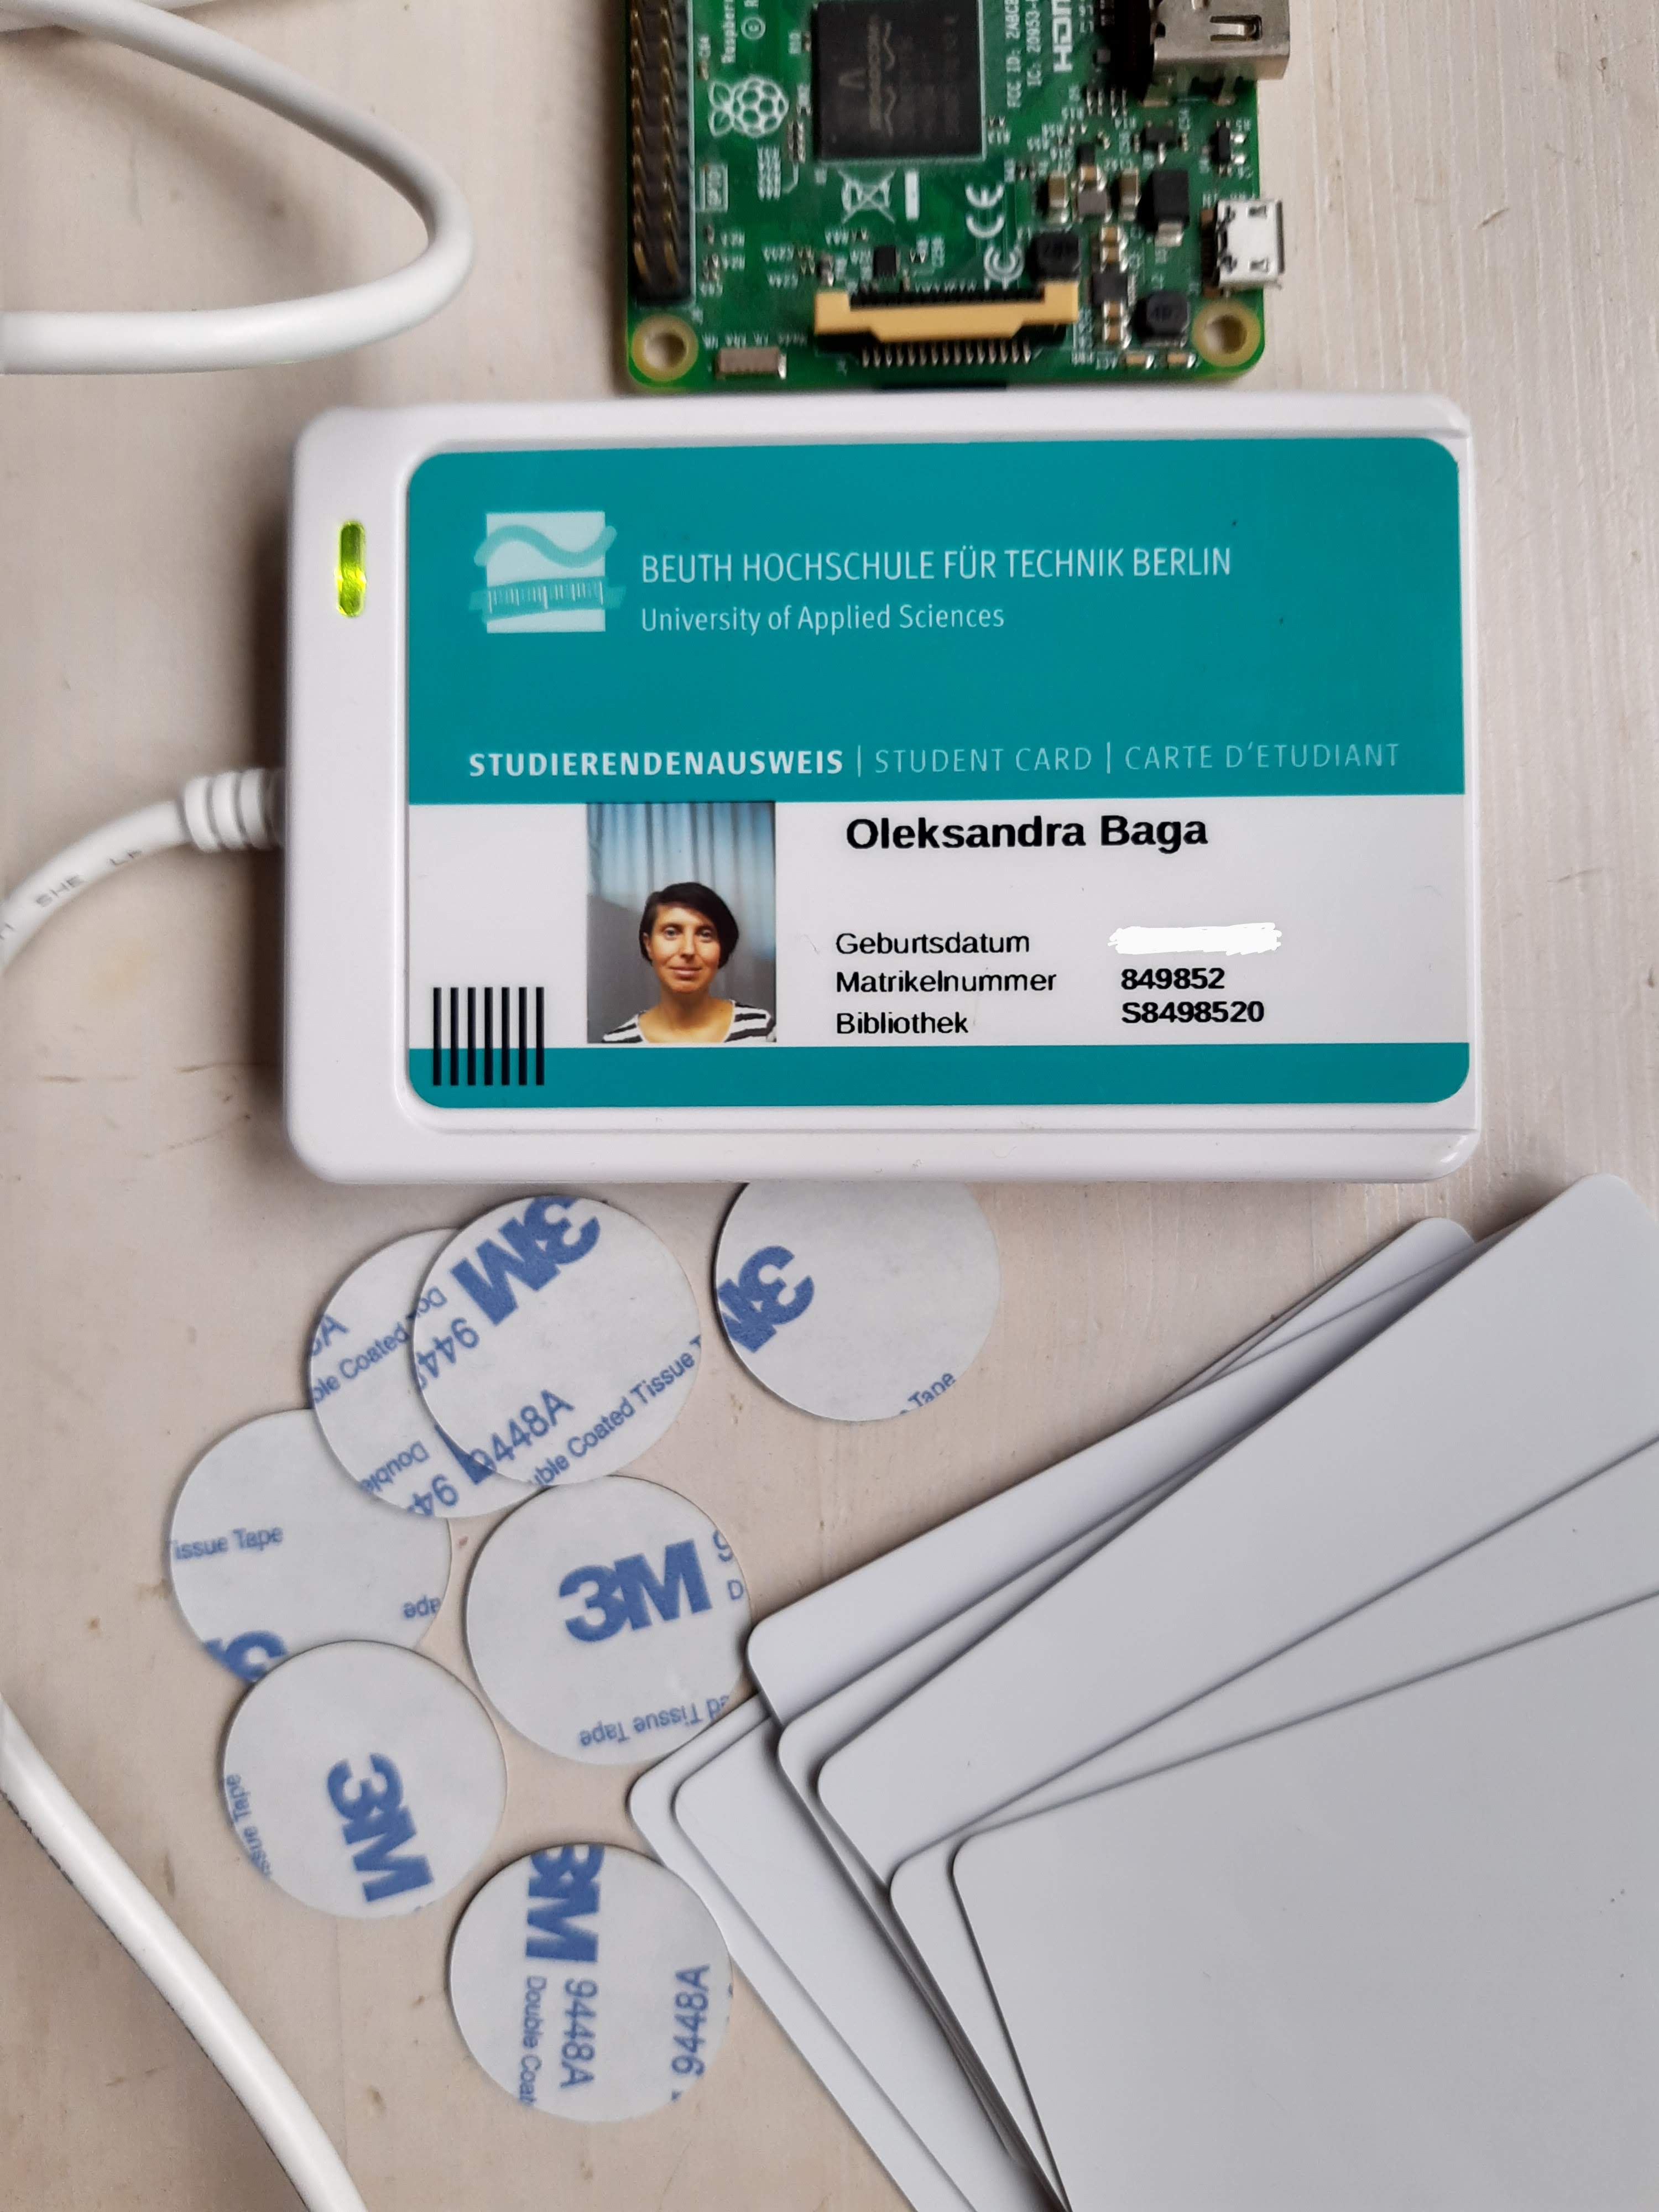
\includegraphics[width=0.42\textwidth]{gfx/baga_stud.jpg}}
	\caption{RFID-Leser mit der Studentenkarte der Autorin und Tags}
	\label{fig:baga_stud}
\end{wrapfigure} 
Wie die weitere Entwicklung darf einfach den ersten gefundenen RFID-Leser genommen werden. Wenn keine Terminals angeschlossen sind, wird das Programm beendet und eine entsprechende Meldung der PSE-Labor Mitarbeiter ausgegeben. Dann muss mit dem ausgewählten Terminal verbunden werden. Dies erfolgt durch Aufrufen der Funktion $SCardConnect()$. Beim Aufruf von $SCardConnect()$ geben wir den gemeinsam genutzten Modus $(SHARE\_SHARED)$, das bevorzugte Kommunikationsprotokoll (in unserem Fall T0 und T1) an, übergeben die Adresse der Variablen, in die das Handle für weitere Operationen mit der Karte gespeichert wird, und die Adresse der Variablen $active\_protocol$. in der gewählten Kommunikationsprotokoll gespeichert wird. Auf Anwendungsebene interessiert es uns nicht besonders, welches Protokoll zum Herstellen der Verbindung ausgewählt wurde, aber diese Informationen müssen während der Programmierung gespeichert werden - sie werden später zum Senden von Befehlen benötigt \cite[p. 104]{chirico:smart_card}.
\begin{lstlisting}[caption={Funktion SCardEstablishContext},captionpos=b]
hresult, hcontext = SCardEstablishContext(SCARD_SCOPE_USER)
	if hresult == SCARD_S_SUCCESS:
		hresult, readers = SCardListReaders(hcontext, [])
		if len(readers) > 0:
			reader = readers[0]
			hresult, hcard, dwActiveProtocol = SCardConnect(hcontext, reader, SCARD_SHARE_SHARED, SCARD_PROTOCOL_T0 | SCARD_PROTOCOL_T1)
\end{lstlisting}

ATR (Answer-To-Reset) ist ein kurzes (nicht mehr als 33) Byte-Array, das die Karte beim Anschließen an das Terminal senden muss. Wenn die Karte dies nicht innerhalb einer bestimmten Zeit tut, wird davon ausgegangen, dass sie nicht richtig funktioniert. ATR enthält grundlegende Informationen über die Karte und die technischen Parameter der Verbindung. Das Format ist jedoch recht kompliziert und hängt vom Hersteller des Kartenchips, den darauf installierten „Anwendungen“ usw. ab. ATR wird im Terminal gespeichert, solange die Karte angeschlossen ist. Es lässt sich die zwei verschiedenen RFID-Transponder (MIFARE Smart-Studentenkarte und RFID-Tag) mit Hilfe ATR voneinander unterscheiden. Das folgendes wird z.B. von der Studentenkarte zurückbekommen, wann Autorin ihre eigene Studentenkarte am RFID-Leser ablesen lässt (siehe Abbildung \ref{fig:baga_stud}):
\begin{lstlisting}[caption={Abgelesene Studentenkarte},captionpos=b]
+Inserted:  3B 81 80 01 80 80
Student card added
uid 04 2F 75 7A 30 40 80
\end{lstlisting}

Das anderes wird aber angezeigt, wann den RFID-Transponder am RFID-Leser präsentiert wird, den in der Zukunft am im PSE-Labor vorhandenen Raspi-Boards angeklebt wird:
\begin{lstlisting}[caption={Abgelesener Raspi-Tag},captionpos=b]
+Inserted:  3B8F8001804F0CA000000306030001000000006A
Raspi board added
uid 5C E7 87 30
\end{lstlisting}

Klasse $DetectionObserver$ mit der Vererbung vom der Klasse $CardObserver$ wird benutzt, um zu erkennen, wann eine Karte dem Kartenleser vorgelegt wurde, und dann die eindeutige Kennung (UID) von einer Karte zu lesen. Es wird mithilfe der Klasse $ CardMonitor$ getan, die das Einsetzen / Entfernen von Smartcards überwacht und den $CardObserver$ benachrichtigt. 
\begin{lstlisting}[caption={Monitor der angelegte und enfertne Smartkarten},captionpos=b]
def update(self, observable, actions):
	(addedcards, removedcards) = actions
	for card in addedcards:
		atr = toHexString(card.atr)
		added_card = self.get_cardtype(toHexString(card.atr), "added")
		self.read_uid(added_card)
\end{lstlisting}

Sobald eine korrekte Studentenkarte oder RFID-Transponder am RFID-Leser erscheint und ohne Kollision mit anderen in der Nähe bleibenden elektromagnetische Felde abgelesen wird, wird abhängig vom dem Typ der Karte eine JSON-Datei erstellt und von einem acaLoan-client zum Server geschickt. Der acaLoan-client selbst ist ein kleinen Python-Script, der die korrekte Erstellung der JSON-Datei erlaubt und eine Verbindung mittels HTTP-Protokoll zum Server bedient. 
\begin{lstlisting}[caption={acaLoanClient},captionpos=b]
class AcaLoanClient:
	def __init__(self, base_url):
		self.base_url = base_url
	
	def send_event(self, type, uid):
		endpoint = "{}/loan/api/events".format(self.base_url)
		payload = {"type": type, "uid": uid}
		r = requests.post(endpoint, json=payload)
\end{lstlisting}

Es wird weiteres von Register-Client auf keine Antwort vom Server erwartet, ob der abgelesenen Studentenkarte die Ausleihe des Raspi-Boards erlaubt ist oder ob gehaltenen in der Hand Raspi-Board ausgeliehen oder zurückgegeben darf. Sobald die Verbindung zum Server erfolgreich hergestellt wurde und eine JSON-Datei geschickt, wird der RFID-Leser wieder zum Ablesen der nächsten RFID-Transponder freigegeben. Der Python-Script für RFID-Leser muss am Register-Client mit der Verwendung der Umgebungsvariable $LOAN_SERVER$. Während der Entwicklung der Abschlussarbeit geschieht es mit dem Name des Django Entwicklungsservers. Mehr darüber ist in folgenden Kapitel \ref{sec:server} nachzulesen.
\begin{lstlisting}[caption={[Umgebungsvariable für den Serverstart] },captionpos=b]
LOAN_SERVER_URL=http://127.0.0.1:8000 python reader.py
\end{lstlisting}
Als letztes für die Implementierung des Register-Clients ist es wichtig, die kurze Beschreibung der entwickelte von Autorin JSON-Datei anzugeben. Definition der Struktur, des Inhalts und der Semantik von JSON-Objekten geschieht mithilfe von der Grammatiksprache namens JSON-Schema. Hier kann Metadaten (Daten über die Daten) angegeben werden, die die Eigenschaften eines Objekts beschreiben und gültige Werte. 

\begin{lstlisting}[caption={JSON-Schema},captionpos=b]
{"$schema": "http://json-schema.org/draft-04/schema#",
"type": "array", "items": [
	{"type": "object", "properties": {
		"type": {"type": "string",
			"enum": ["card", "uid", "cancel_button", "terminate_button", "get_rfid_status",
			"return_scanned_board_button", "loan_scanned_board_button", "finish_button"]},
		"uid": {"type": "string"}},
	"required": ["type", "uid"]}]}
\end{lstlisting}

Zu Zweck Definition der Struktur wird das Schlüsselwort "items" mit einem Array gesetzt, wobei jedes Element ein Schema ist, das jedem Index des Arrays des Dokuments entspricht. Das heißt, ein Array, bei dem das erste Element das erste Element des Eingabearrays validiert, das zweite Element das zweite Element des Eingabearrays validiert usw \cite{website:14}. Es ist zu betonen, dass für das ersten Element der JSON-Datei es eine Zeichenfolge aus einem festen Wertesatz sein muss. Nur diesen Zeichenfolgen können von Endliche Zustandsmaschine, die im Kapitels \ref{sec:design:fsm} und \ref{sec:server:restapi} beschrieben sind, abgearbeitet werden. 

\section{Server}
\label{sec:server}
Als er wurde im Kapitel \ref{sec:register_client:smart} erwähnt, während der Implementierung der Aufgabe der Abschlussarbeit wurde mit dem Entwicklungsserver gearbeitet. Ein Entwicklungsserver ist ein Servertyp, der die Entwicklung und das Testen von Programmen, Websites, Software oder Anwendungen für Softwareprogrammierer erleichtert. Der bietet eine Laufzeitumgebung sowie alle Hardware- / Software-Dienstprogramme, die für das Debuggen und die Entwicklung von Programmen unerlässlich sind. Django ist eines der effizientesten modernen Frameworks für die Entwicklung von Webprojekten. Der Grund für diese Effizienz ist ein klarer Mechanismus für die Arbeit mit einem Projekt, ein praktisches ORM (Object Relational Mapping Layer), mit der mit Anwendungsdaten aus verschiedenen relationalen Datenbanken wie SQLite, PostgreSQL und MySQL interagiert werden kann.

\subsection{Erstellung acaLoan Django-Projekts}
\label{sec:server:install}
Glücklicherweise ist der Installationsprozess für Django unkompliziert, sodass das Einrichten Ihrer Entwicklungsumgebung schnell und entspannt ist. Django ist vollständig in Python geschrieben, daher muss zuerst Python installiert werden, um Django zu installieren. Weil die Autorin für die Implementierung des Servers ihren eignen Mac OS Rechner verwendet, ist Python bereits Computer installiert. Wenn "Python" in die Befehlszeile eingegeben (mithilfe der Terminal.app auf meinem Mac), wurde folgendes angezeigt werden:
\begin{lstlisting}[caption={[Python Version überprüfen ] },captionpos=b]
$ python
Python 3.8.1 (default, Feb 17 2020, 23:55:16) 
[Clang 11.0.0 (clang-1100.0.33.17)] on darwin
\end{lstlisting}

Sobald Python auf Computer installiert ist, kann Django auch installiert werden. Es gibt drei Möglichkeiten: Installation der offizielle Django-Version, Verwendung eines verteilungsspezifisches Installationsprogramm oder Herunterladen der Version, die derzeit immer noch entwickelt wird. In der Abschlussarbeit wird nur die Installation der offiziellen Version verwendet. Der Installation wird mit "Pipenv"-Tool geschieht, das isolierte Python-Umgebungen bietet, die somit praktischer sind als die systemweite Installation von Paketen. Pipenv verwaltet Projektpakete automatisch über die Pipfile-Datei, während die Pakete installiert oder deinstalliert werden. Pipenv generiert auch die Datei Pipfile.lock, mit der deterministische Builds erstellt und eine Momentaufnahme Ihrer Arbeitsumgebung erstellt werden. Zusätzlich für die Aufgabeimplementierung wird django-fsm installiert, das mit der Django Installation nicht geliefert wird und erlaubt eine einfache deklarative Zustandsverwaltung für Django-Modelle. 

Der ganzen Quellcode für das acaLoan-Server wird als Django Projekt dargestellt. Django hat einen Befehl zum einfachen Erstellen einer anfänglichen Projektstruktur. Es wird mit der Ausführung des folgenden Befehls vom Terminal erledigt:
\begin{lstlisting}[caption={[Erstellung acaLoan Django-Projekts] },captionpos=b]
 django-admin startproject acaLoanRaspiBoard   
\end{lstlisting}

\begin{figure}
	\centering
	\fbox{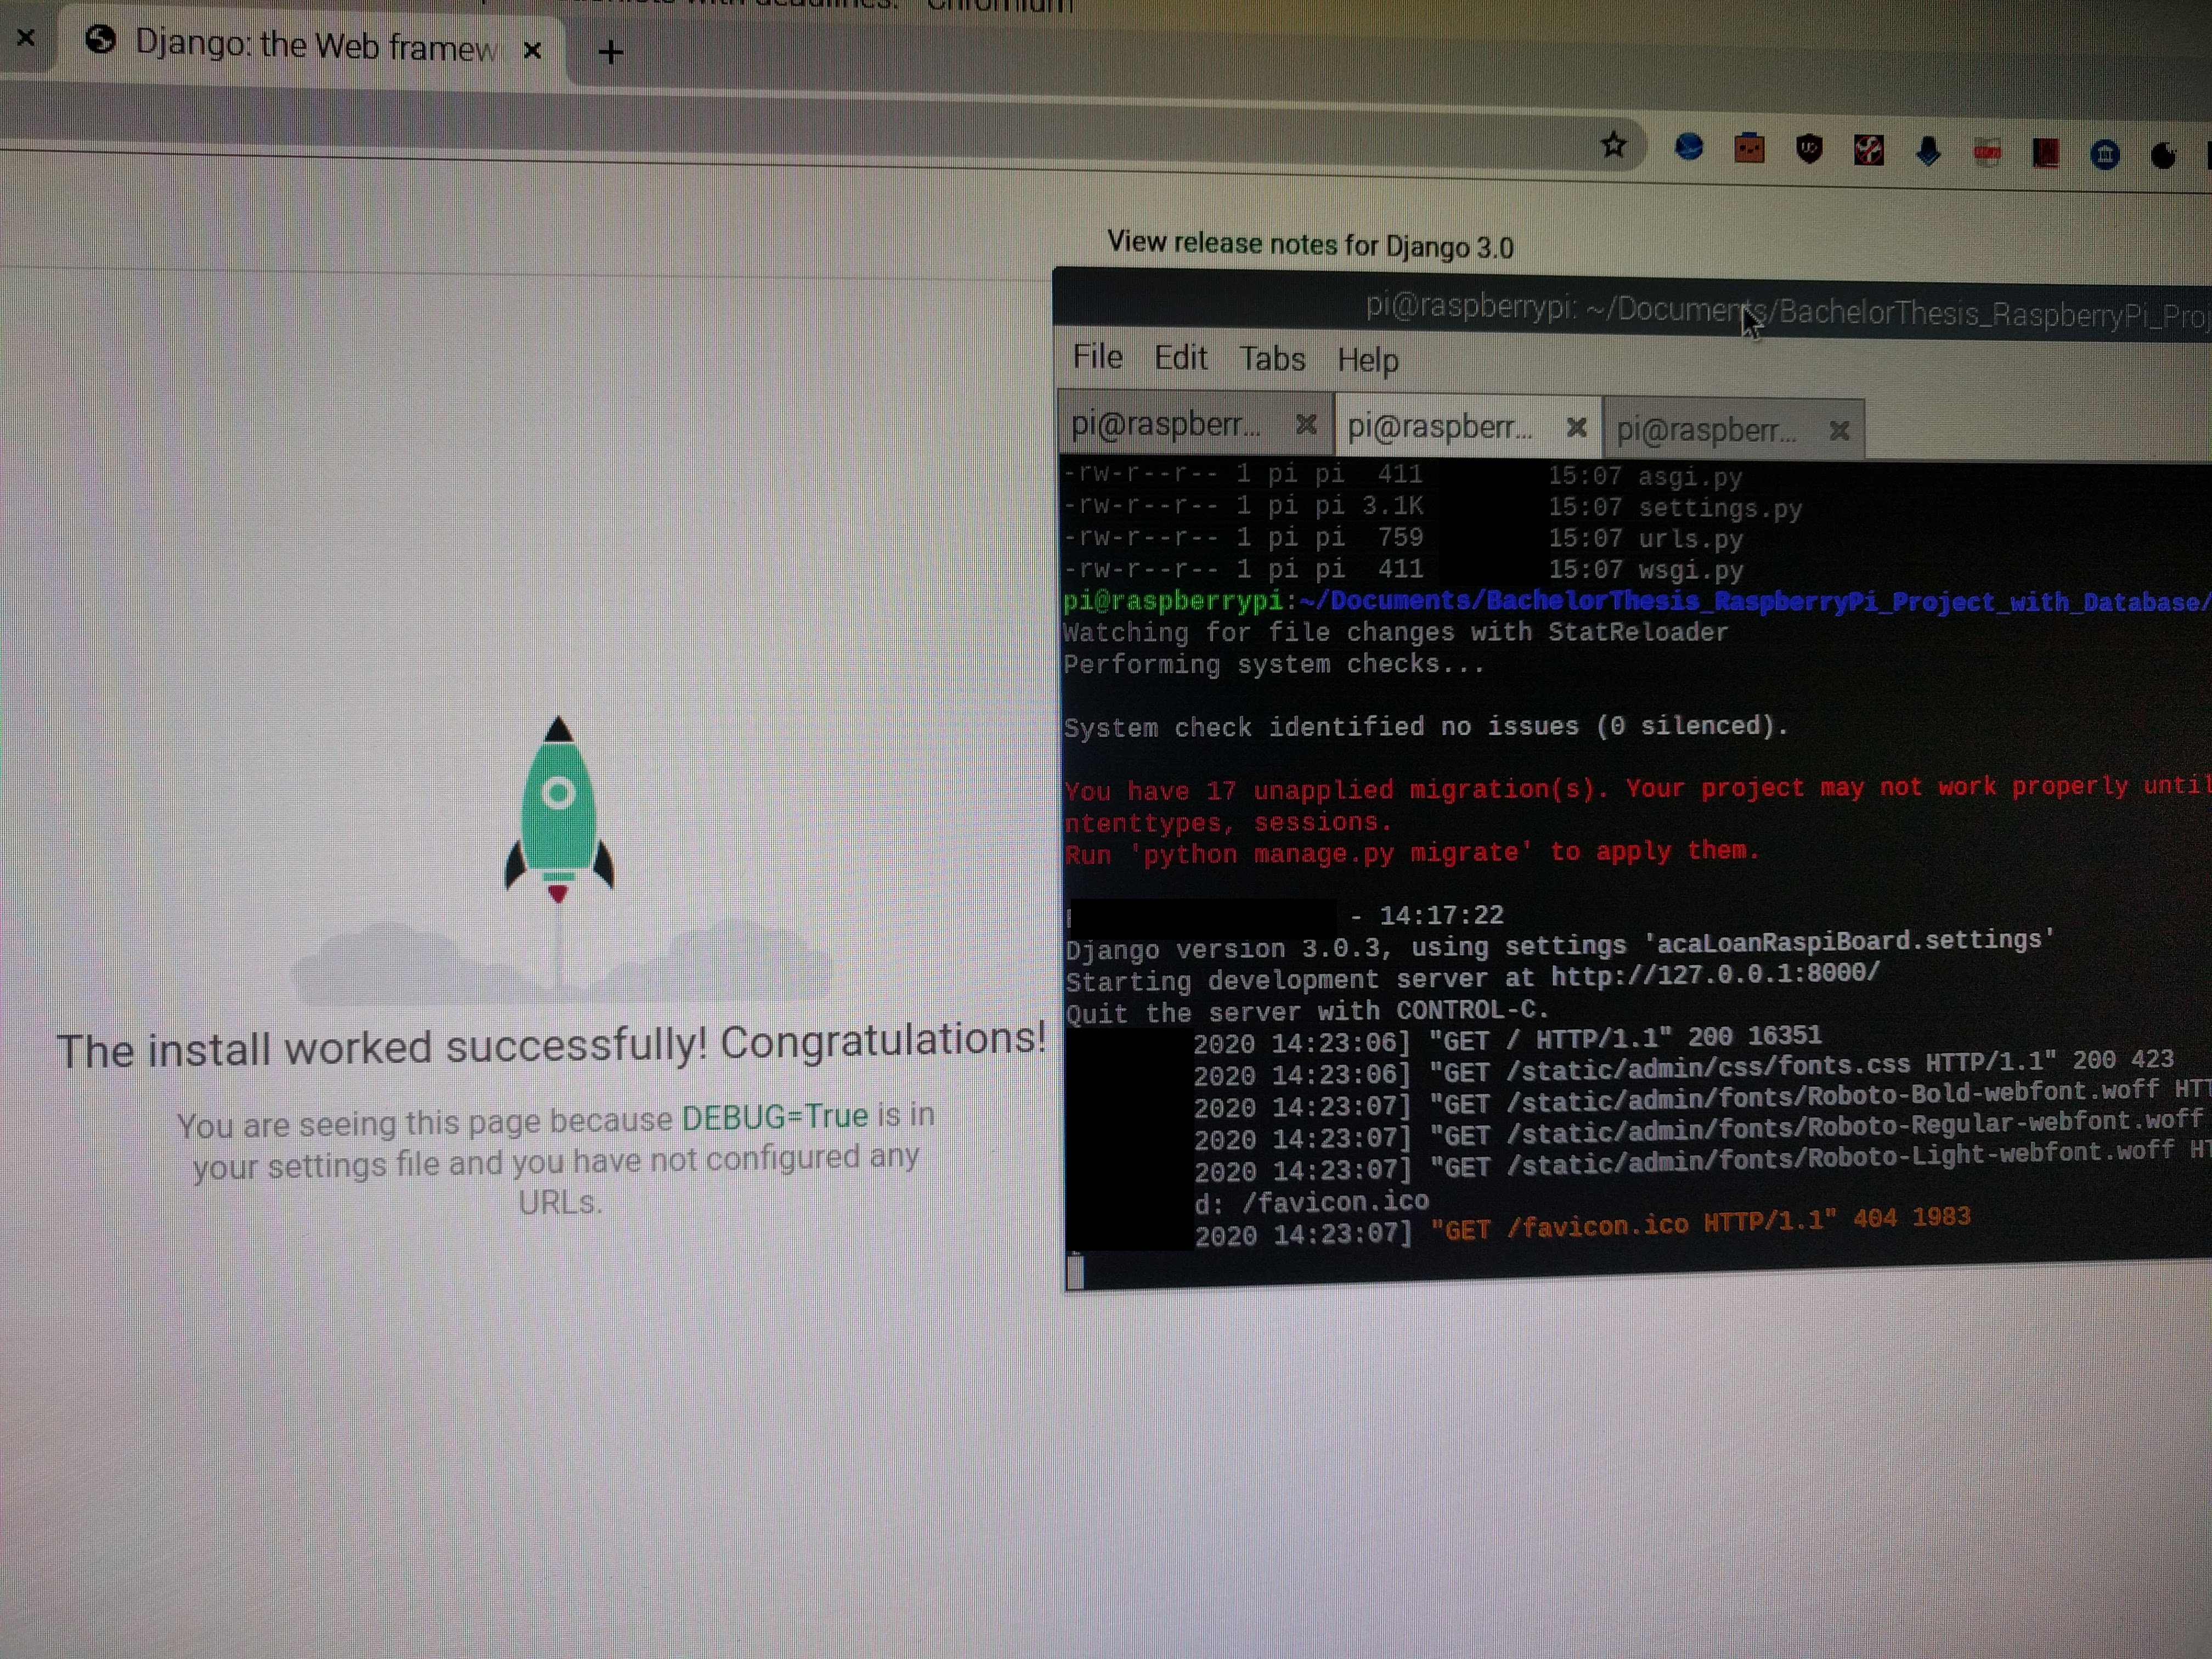
\includegraphics[width=1\textwidth]{gfx/django_start.jpg}}
	\caption{Server nach Erstellung des acaLoanRaspiBoard-Projekts}
	\label{fig:django_start}
\end{figure}

Die Datei settings.py enthält eine Grundkonfiguration für die Verwendung einer SQLite-Datenbank und eine Liste von Django-Anwendungen und wurde als während der Implementierung geändert, um das üblichste deutsche Zeitformat anstatt des amerikanischen zu verwenden.
\begin{lstlisting}[caption={Deutsches Zeitformat in Django},captionpos=b]
LANGUAGE_CODE = 'en-us'
TIME_ZONE = 'Europe/Berlin'
TIME_INPUT_FORMATS = ['%H:%M:%S']
TIME_FORMAT = '%H:%M:%S'
DATETIME_FORMAT = "d.m.Y H:m"
DATE_FORMAT = "Y-m-d"
\end{lstlisting}
acaLoan-Server muss im zusätzliche Dateien wie Bilder, JavaScript oder CSS bereitstellen. In Django werden diese Dateien als "statische Dateien" bezeichnet. Django stellt django.contrib.staticfiles zur Verfügung, um den Entwickler bei der Verwaltung zu unterstützen. Dafür müssen in die Datei settings.py die folgenden Zeilen hinzugefügt werden:
\begin{lstlisting}[caption={[Die zusätzliche Dateien in das Projekt hinzufügen] },captionpos=b]
STATIC_URL = '/static/'
STATICFILES_DIRS = [os.path.join(BASE_DIR, "staticfiles")]
\end{lstlisting}

In der settings.py ist auch den Debug-Modus des Projekts aktiviert, um während der Entwicklung detaillierte Fehlermeldungen zu sehen.  Nach der Erstellung des Projekts und kleine notwendigen Änderungen, kann endlich acaLoan-Server gestartet werden. Da Django einen praktischen Mechanismus bietet, um die Konfiguration Ihres Webservers während der Entwicklung zu vermeiden, kann enthaltenen bereits ein Webserver mit dem Befehl aufgerufen werden: 
\begin{lstlisting}[caption={[runserver-Befehl] },captionpos=b]
python manage.py runserver
\end{lstlisting}
Nach dem Befehl ausgeführt wurde und im Browser zu http://127.0.0.1:8000/ navigiert wurde, wird die folgende Ausgabe angezeigt, die auf der Abbildung \ref{fig:django_start} zu sehen ist.
 
\subsection{Datenbankeinrichtung}
\label{sec:server:database}
Nach dem Erstellung des Projekts und dem ersten Starten des acaLoan-Server ist es die Zeit, sich mit der Einrichtung von Datenbank zu beschäftigen. Theoretisch kann ein Django-basierte Projekt ohne Datenbank ausgeführt werden. Für die hier vorliegenden Abschlussarbeit was jedoch es ein Zweck, eine Datenbank einzurichten, um alle Ausleihe-/Rückgabevorgänge zu verwalten, so dass in einem echten Projekt kann man nicht auf Datenbankeinrichtung verzichten. Für die Implementierung wird für Verwendung von SQLite3 entschieden. Die Datenbank selbst wird in einer Datei auf der Festplatte gespeichert. Um die Datenbank mit dem Django-Projekt zu verbinden, muss den DATABASES-Block in der Datei $mysite/settings.py$ bearbeitet. Um sqlite zu verwenden, muss nur $django.db.backends.sqlite3$ als ENGINE angegeben und den Namen der Datei, in der die Datenbank gespeichert wird, in den Parameter NAME geschrieben werden \cite{website:15}.

Als nächsten müssen die Modelle in Django erzeugt werden, die die Daten definieren, mit denen während der Entwicklung gearbeitet werden. Die Modelle in Django werden entsprechend des Klassendiagramm aus dem Kapitel \ref{sec:design:uml:class} und des Entity Relationship Diagramm realisiert, das im Kapitel \ref{sec:design:db} gezeigt wurde. Die wichtigste Modelle sind unten zu sehen:

\begin{lstlisting}[caption={Student Modell},captionpos=b]
class Student(models.Model):
	student_card = models.OneToOneField(StudentCard, on_delete=models.SET_NULL, blank=True, null=True)
	semester = models.ForeignKey(Semester, on_delete=models.CASCADE, blank=True, null=True)
	first_name = models.CharField('first name', max_length=50)
	second_name = models.CharField('second name', max_length=50)
	matricul_no = models.CharField('matriculation', max_length=10, unique=True)
	hrz_no = models.CharField('hrz', max_length=10, unique=True)
	group = enum.EnumField(StudentGroup)
	is_home_loan_enabled = models.BooleanField(default=True)
\end{lstlisting}
 ForeignKey wird verwendet, um eine Viele-zu-Eins-Beziehung zu definieren, die eine Beziehung zwischen mehr als einer Instanz einer Entität und einer Instanz einer anderen Entität ist. Sodass in der Datenbank für ein Semester können mehrere Studierende immatrikuliert werden. $on\_delete=models.CASCADE$ ist ein SQL-Standard, das nicht nur in Django verwendet wird. Wenn das referenzierte Objekt gelöscht wird, ist auch die Objekte zu löschen, auf die es verwiest. Wenn es beispielsweise einen Semester zu entfernen ist, müssen auch die Studenten gelöscht, die während dieses Semester in System registriert wurden. Damit sollen alle veraltet Daten der Studierende nach dem Semesterende endgültig aus der Datenbank gelöscht werden. 
\begin{lstlisting}[caption={Board Modell},captionpos=b]
class Board(models.Model):
	raspi_tag = models.OneToOneField(RaspiTag, on_delete=models.SET_NULL, blank=True, null=True)
	board_no = models.IntegerField('board number', unique=True)
	board_type = enum.EnumField(BoardType, default=BoardType.LAB_LOAN)
	board_status = enum.EnumField(BoardStatus, default=BoardStatus.ACTIVE)
 \end{lstlisting}
Um eine Eins-zu-Eins-Beziehung zu definieren, wird OneToOneField verwendet. In einer relationalen Datenbank besteht eine Eins-zu-Eins-Beziehung, wenn eine Zeile in einer Tabelle nur mit einer Zeile in einer anderen Tabelle verknüpft sein kann und umgekehrt.
\begin{lstlisting}[caption={Action Modell},captionpos=b]
class Action(models.Model):
	# Holds the record about the loan operation, student, board and time
	student = models.ForeignKey(Student, on_delete=models.SET_NULL, blank=True, null=True)
	board = models.ForeignKey(Board, on_delete=models.SET_NULL, blank=True, null=True)
	timestamp = models.DateTimeField(auto_now=True)
	operation = enum.EnumField(Operation, default=Operation.UNKNOWN_OPERATION)
\end{lstlisting}
Mit $DateTimeField(auto_now=True)$ wird die Zeit der Ausleihe-/Rückgabeaktion genau entsprechend der Zeit des Servers gespeichert. 
\begin{lstlisting}[caption={Session Modell},captionpos=b]
class Session(models.Model):
	# Holds the information about the interaction between user (student) and system
	TERMINAL_STATES = ['timeout', 'finished', 'canceled', 'error_terminated']
	start_time = models.DateTimeField(default=datetime.datetime.now)
	state = FSMField(default='session_started')
	last_action_time = models.DateTimeField(auto_now=True)
	student_card = models.ForeignKey(StudentCard, on_delete=models.SET_NULL, blank=True, null=True, related_name='+')
	raspi_tag = models.ForeignKey(RaspiTag, on_delete=models.SET_NULL, blank=True, null=True, related_name='+')
\end{lstlisting}
An dieser Stelle muss man besonders betonen, dass Feld $state = FSMField(default='session\_started')$ wird für Django Finite State Machine Framework benutzt. Anstatt einem Django-Modell ein Statusfeld hinzuzufügen und seine Werte manuell zu verwalten, wird FSMField verwendet und Modellmethoden mit dem Übergangsdekorator markiert \cite{website:fsm}. Diese Methoden können Änderungen der Zustandsänderung enthalten. Die Implementierung wird in Kapitel \ref{sec:server:fsm:fsm} erklärt. Nachdem die Django Modelle entsprechend der Beschreibung aus dem Kapitel \ref{sec:design:uml:class} erzeugen wurden, müssen die Tabellen in der Datenbank erstellt werden, bevor sie verwendt werden können. Dazu wird den  Befehl ausgeführt:
\begin{lstlisting}[caption={[Der Befehl migrate] },captionpos=b]
$ python manage.py migrate
\end{lstlisting}
Der Befehl migrate überprüft die Einstellung $INSTALLED\_APPS$ und erstellt alle erforderlichen Datenbanktabellen gemäß den Datenbankeinstellungen in der Datei $acaLoanRaspiBoard/settings.py$ \cite{website:15}.

\subsection{Einführung in das Django Admin}
\label{sec:server:admin}
\begin{figure}
	\centering
	\fbox{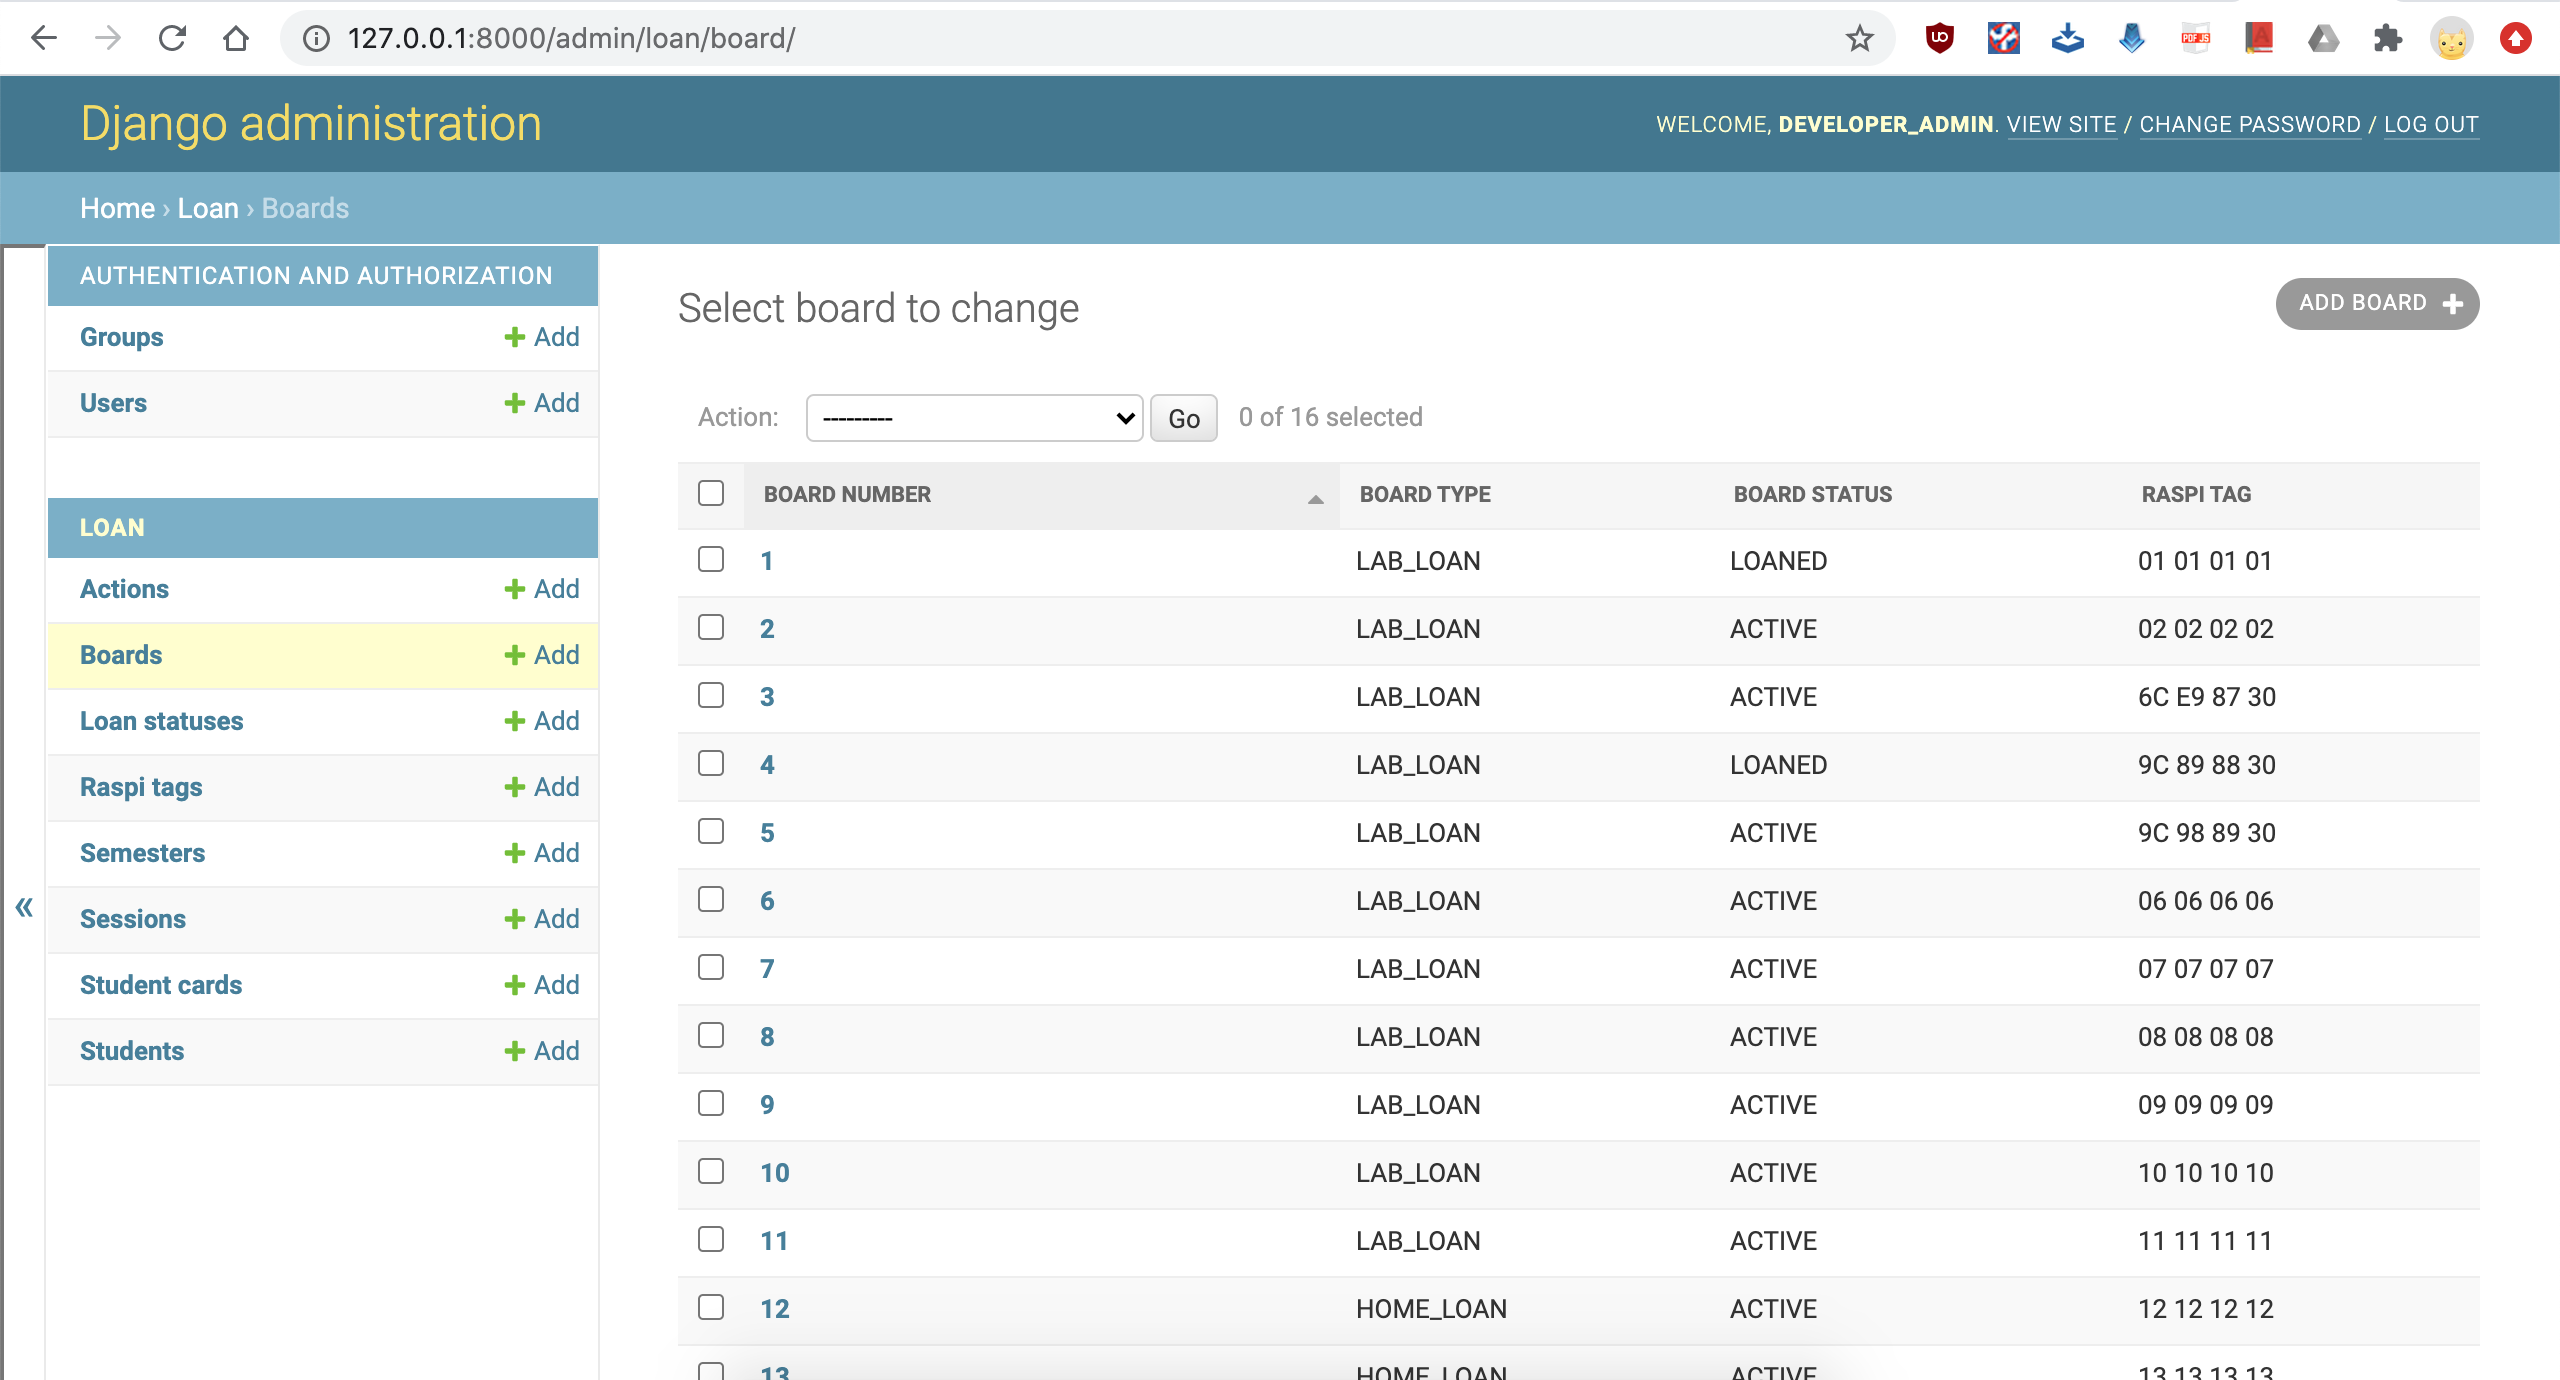
\includegraphics[width=1\textwidth]{gfx/django_admin.png}}
	\caption{Screenshot von Django Admin Site mit Board Tabelle.}
	\label{fig:django_admin}
\end{figure}
Einer der mächtigsten Teile von Django ist die automatische Administrationsoberfläche. Es liest Metadaten aus erstellten Modellen, um eine schnelle, modellzentrierte Oberfläche bereitzustellen, über die vertrauenswürdige Benutzer Inhalte auf der Website verwalten können \cite{website:djangoAdmin}. Die Admin-Site verwendet werden kann, indem die URL aufgerufen wird, mit der Die Admin-Site verbunden wurde (im AcaLoan-Projekt ist es $/admin/$). Wenn einen Benutzer zum Anmelden erstellt werden muss, wird es mit dem Befehl createuperuser gemacht. Für die Anmeldung beim Administrator muss der Benutzer standardmäßig das Attribut $is\_superuser$ oder $is\_staff$ auf True gesetzt haben. Mithilfe der Django-Admin Site können die Mitarbeiter nicht benutzerorientierten Inhalt verwalten. Z.B. so werden am Anfang jedes Semesters die neuen Datensätzen für die registrierten für das Modul Studierende erstellt. 
\begin{wrapfigure}{l}{0.45\textwidth}
	\fbox{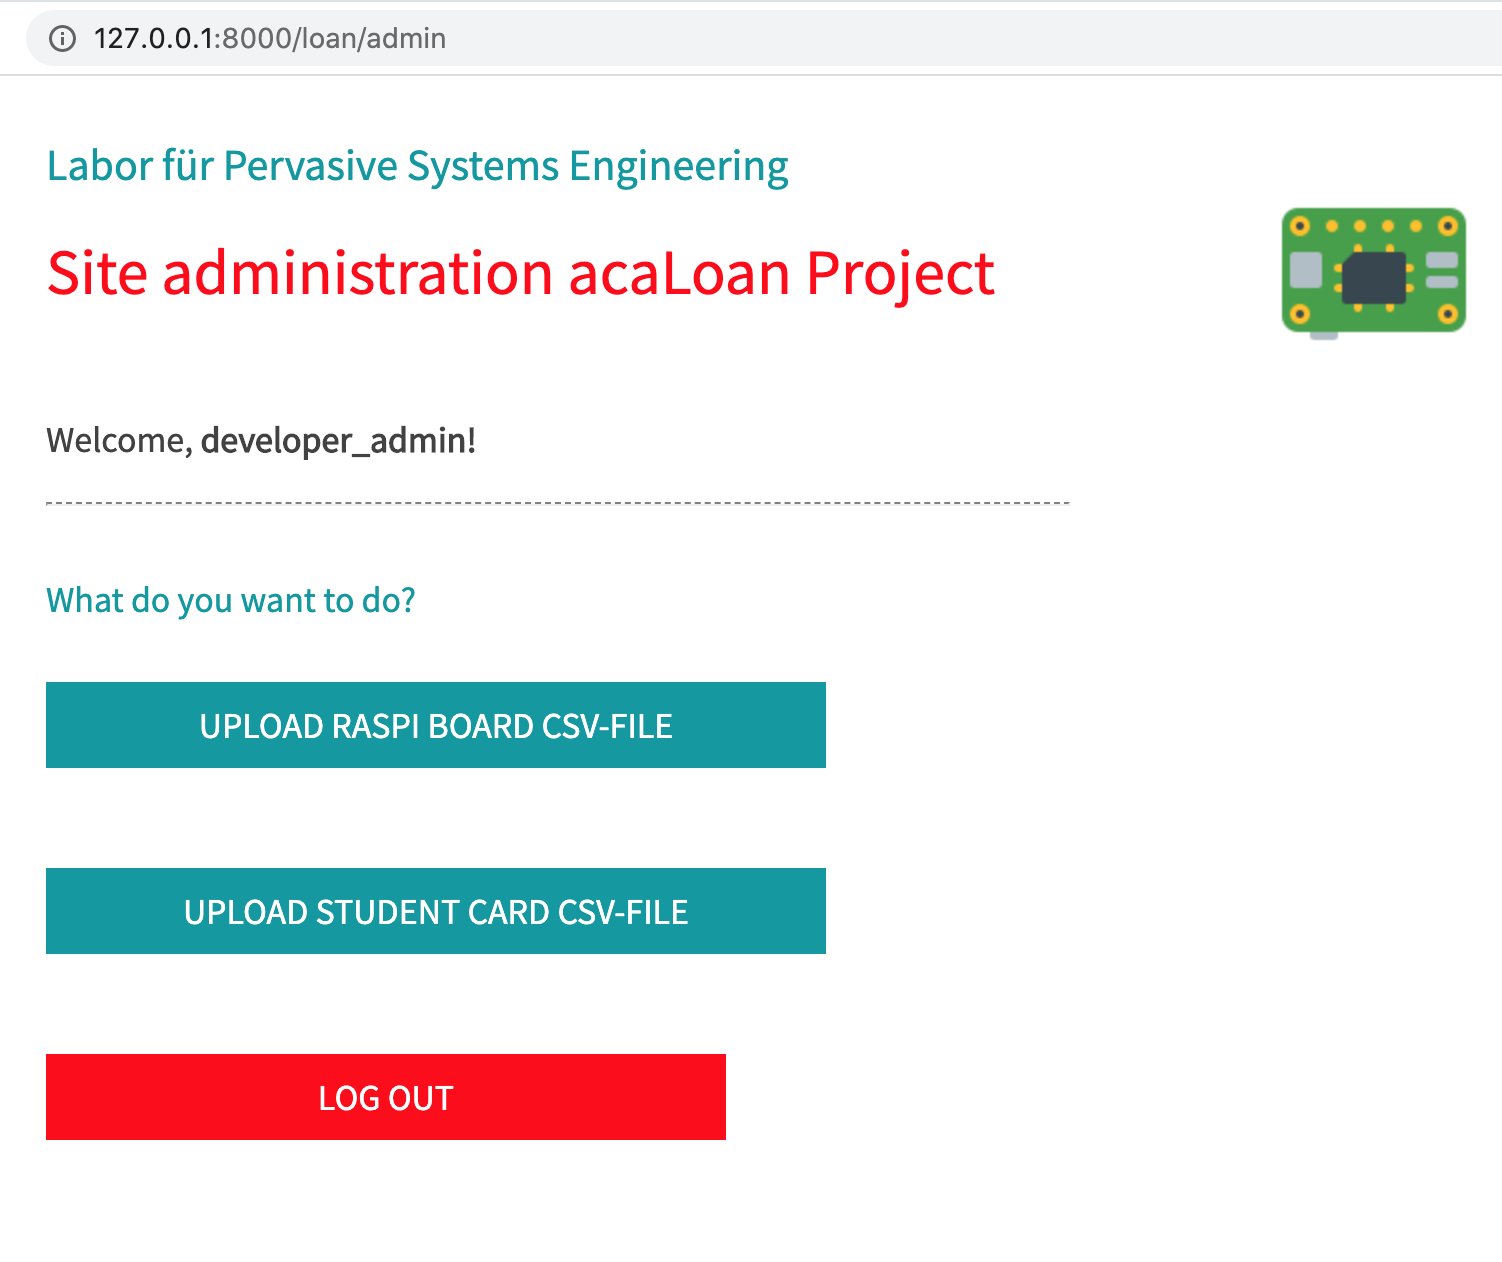
\includegraphics[width=0.42\textwidth]{gfx/upload_csv.png}}
	\caption{Admin spezifische Site für CSV-Hochladen}
	\label{fig:upload_csv}
\end{wrapfigure}
Um einen  Arbeitszeitverbrauch des Mitarbeiter des PSE-Labor zu senken, wurde das kleine Python Script geschrieben, das permanenten Identifikationsnummer (UID) von einer kontaktlosen Speicherkarte der Studierende ablesen und als CSV-Datei auf der Festplatte speichern kann. Nachdem die Datensätze der Studierende in der Datenbank erzeugen und die UIDs mithilfe des Scripts am RFID-Leser abgelesen wurden, kann Admin des acaLoan-Systems die CSV-Datei hochladen. Somit werden die UIDs der Studentenkarten automatisch mit dazugehörigen Studentensätzen über eindeutigen Matrikelnummer verknüpft. Die Seite mit dem Hochladen der CSV-Datei ist nur für den vertrauenswürdigen Admin des System zu Verfügung stehen dürfen und den Zugriffsrechten sind von Django zu verwalten, dazu den entsprechenden Schnittstelle mit dem $@staff\_member\_required$ geschützt wird geworden.

\subsection{Design der acaLoan-Website}
\label{sec:server:design}
\begin{figure}
	\centering
	\fbox{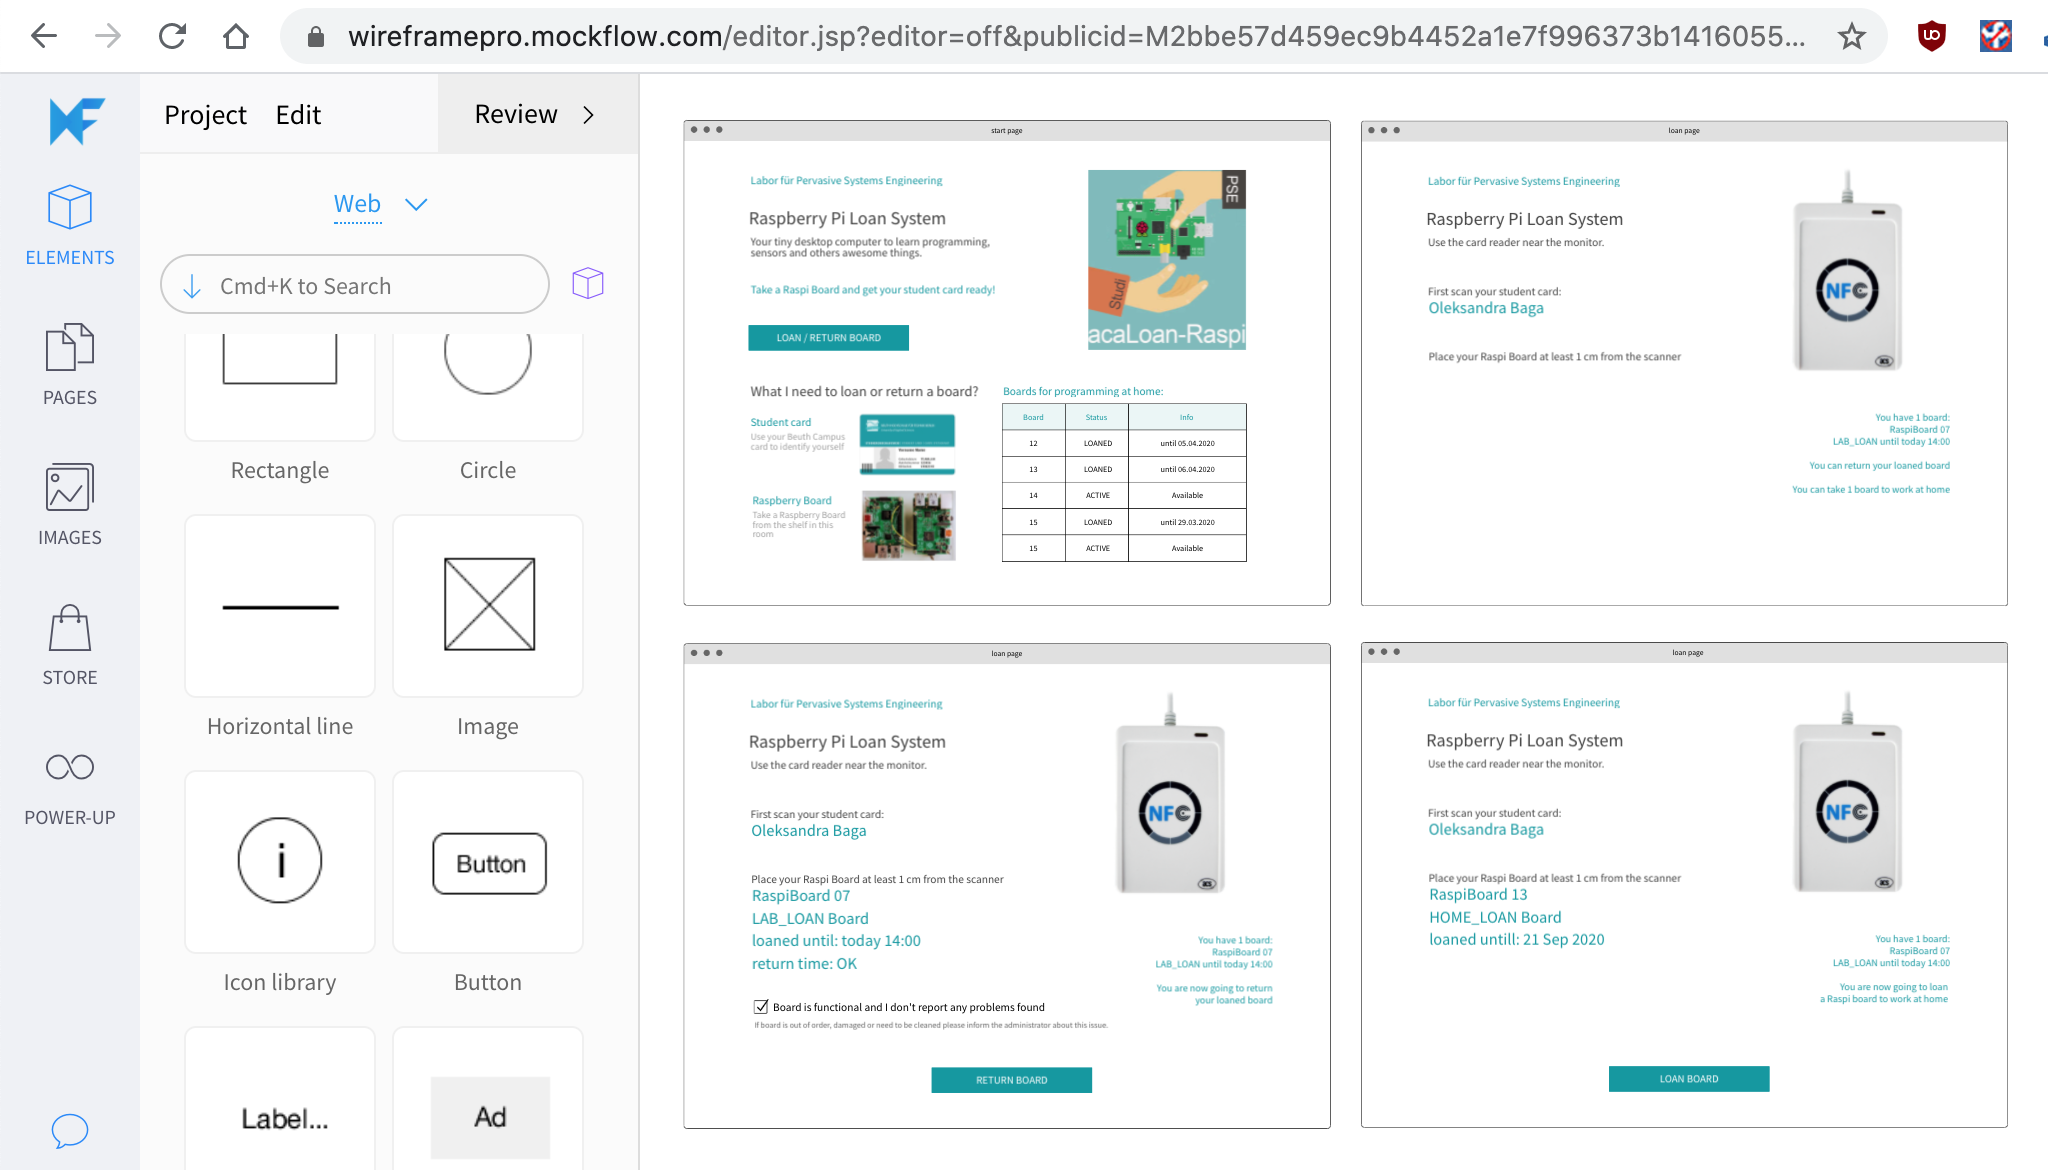
\includegraphics[width=1\textwidth]{gfx/design.png}}
	\caption{Screenshot von mockflow.com mit dem Design}
	\label{fig:design}
\end{figure}
Django wird als Framework für die Erstellung vollständiger Websites benutzt. Das Rendern von HTML ist eine der grundlegenden Fähigkeiten von Django. Da das Design für Display-Client erstellt werden muss, wurde der Styl der Beuth Hochschule für Farben und Schriftarten verwendet ein einfaches Website-Design im kostenlosen Online-Tool "mockflow.com" erstellt. Die Seiten sind auf der Abbildung \ref{fig:design} abgebildet. Dann wurden aus dem Design-Bilder direkt ohne automatisierten Dienste die HTML- und CSS-Dateien erstellt, die später mit Django HTML-Vorlagen verwenden werden.  
\subsubsection{Erstellen der öffentlichen Schnittstelle}
\label{sec:server:design:views}
Nach dem Speichern der HTML- und CSS-Dateien in $/loan/templates$ gespeichert wurden, müssen  die entsprechenden Ansichten erstellt werden, um die Seiten zu rendern. Eine Ansicht ist eine spezifische Webseite in der Django-Anwendung, die bestimmte Funktion erfüllt und über eine bestimmte Vorlage verfügbar ist \cite{website:166:temp}. Sie werden durch eine Python-Funktion (oder eine Methode bei klassenbasierten Ansichten) dargestellt. Django wählt eine Ansicht aus, indem er die angeforderte URL überprüft (genauer gesagt den Teil der URL nach dem Domainnamen) \cite{website:166:temp}. Mit der Ansicht "index" wird acaLoan-Projekt beim Starten ausgeführt und ihre HTML-Vorlage wird dem Benutzer im Webbrowser im Vollbildmodus angezeigt. Mit dem Drücken der Taste "Loan/Return Board" wird eine neue Sitzung in dem Zustand $session\_started$ angefangen. 
\begin{lstlisting}[caption={Index-Ansicht in Django},captionpos=b]
def index(request):
	now = datetime.datetime.now()
	loans = []
	for b in Board.objects.filter(board_no__gte=HOME_LOAN_MINIMAL_NO):	
		if b.board_status == BoardStatus.LOANED:
		action = b.action_set.order_by("-timestamp").first()
		deadline = action.timestamp + MAX_HOME_LOAN_LIMIT	
			if deadline > now:
			loans.append({'board': b, 'deadline': deadline})
		else:
		loans.append({'board': b, 'deadline': None})	
	template_name = "loan/index.html"
	context = {"loans": loans}
	return render(request, template_name, context)
\end{lstlisting}
Hier will ich besonders zeigen, dass in intelligente HTML-Seite die die Variablen anstelle bestimmter Werte verwendet werden kann, um in $index.html$ die verfügbare zur Home-Ausleihe Boards dem Studierende anzuzeigen zu können. Hier werden die verfügbare im Labor Home-Boards und die Boards, deren Rückgabefrist ist immer noch nicht versäumt, aus der Datenbank zugreifen und als Python-Wörterbuch mit Variablennamen der HTML-Vorlage zum rendern übergeben (Abbildung \ref{fig:loaned}). In der Vorlage namens "start" wird den Zustand der Sitzung angezeigt, den wird vom Server über die REST API Kommunikationsschnittstelle dem Display-Client geschickt, die regelmäß abgerufen werden muss. Die Sitzungsaktualisierungen werden in der events-Ansicht behandelt. Zuerst wird es überprüft, ob angekommenen JSON-Datei eine erwartete von dem Server Nachricht erhält. 

\begin{lstlisting}[caption={Events-Ansicht in Django, JSON-Parsing},captionpos=b]
    if request.method != "POST":
		return HttpResponseNotFound()
	...
	try:
		body = json.loads(request.body)
		input_type = body['type']
	except (KeyError, json.JSONDecodeError):
		return HttpResponseBadRequest()	
	if input_type not in ["card", "tag", "cancel_button", "terminate_button", "get_rfid_status",
	"return_scanned_board_button", "loan_scanned_board_button", "finish_button"]:
		return HttpResponseBadRequest()
\end{lstlisting}
Falls die JSON-Datei korrekt ist, wird ihre Inhalt für die Übergang der endlichen Zustandsmaschine verwendet. Es wird detaillierter im Kapitel "Endliche Zustandsmaschine mit Django FSM" erklärt.
\begin{lstlisting}[caption={Events-Ansicht in Django, Aufur von FSM Transitions},captionpos=b]
if input_type == "card":
try:
	uid = body['uid']
	session.student_card_inserted(uid)
except StudentCard.DoesNotExist:
	pass
elif input_type == "tag":
	uid = body['uid']
	session.rfid_inserted(uid)
elif input_type == "cancel_button":
	session.session_canceled()
...
\end{lstlisting}

\subsubsection{Django HTML-Vorlage}
\label{sec:server:design:templates}
Als es im Kapitel oben schon erwähnt wurde, wird von einer Django-Ansicht ein Kontext wie ein Python-Wörterbuch mit Variablennamen als Schlüssel und deren Werten als Wert erzeugt und in die Django HTML-Vorlage übergeben. Beispielsweise ist auf der Abbildung \ref{fig:loaned} die Tabelle mit Home-Loan Boards gezeigt, die im Labor vorhanden sind oder auf dessen baldige Rückkehr erwartet ist. Den Inhalt der Tabelle wurde als ein Kontext aus der Index-Ansicht übergeben und dynamisch generiert. Django unterstützt Jinja, die eine Erweiterung von HTML ist, mit der Daten mit einer doppelten Klammer $\{\{data\}\}$ und Ausdrücke mit ähnlicher Syntax $\{\% expression\%\}$ eingefügt werden können.

\begin{lstlisting}[caption={Django Template Sprache in index.html},captionpos=b]

<tr>
	<td>{{ loan.board.board_no }}</td>
	<td>{{ loan.board.board_status }}</td>
	<td>
		
			Ready to loan
		
		
			
				Loaned until {{ loan.deadline }}
			
		
...
\end{lstlisting}

\begin{figure}
	\centering
	\fbox{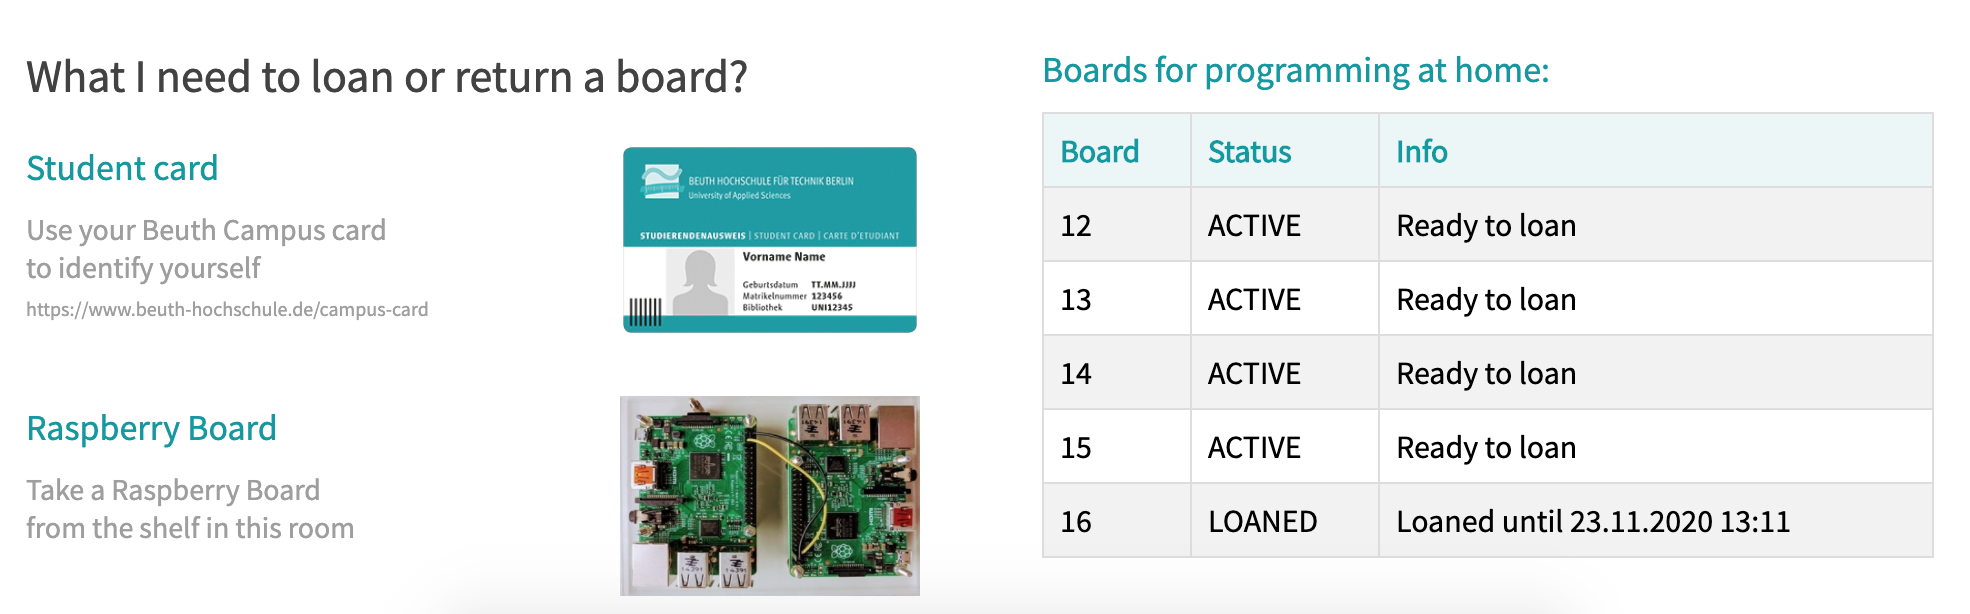
\includegraphics[width=1\textwidth]{gfx/loaned.png}}
	\caption{Teil der Index-Seite: dynamische generierte Tabelle mit verfügbaren im Labor Home-Loan Boards}
	\label{fig:loaned}
\end{figure}

\subsection{Implementierung des Anwendungsfällen}
\label{sec:server:fsm}
Vor der Implementierung der User Cases wurde auch Sequenzdiagramm erzeugt, die einfach die Interaktionen zwischen Objekten in einer sequentiellen Reihenfolge zeigt, d.h. die Reihenfolge, in der diese Wechselwirkungen stattfinden. Die Sequenzdiagramm wurde als nächstes als eine Basis für das Design des Zustandsmaschine verwendet.  

\subsubsection{Sequenzdiagramm}
\label{sec:server:fsm:sequenz}
\begin{figure}
	\centering
	\fbox{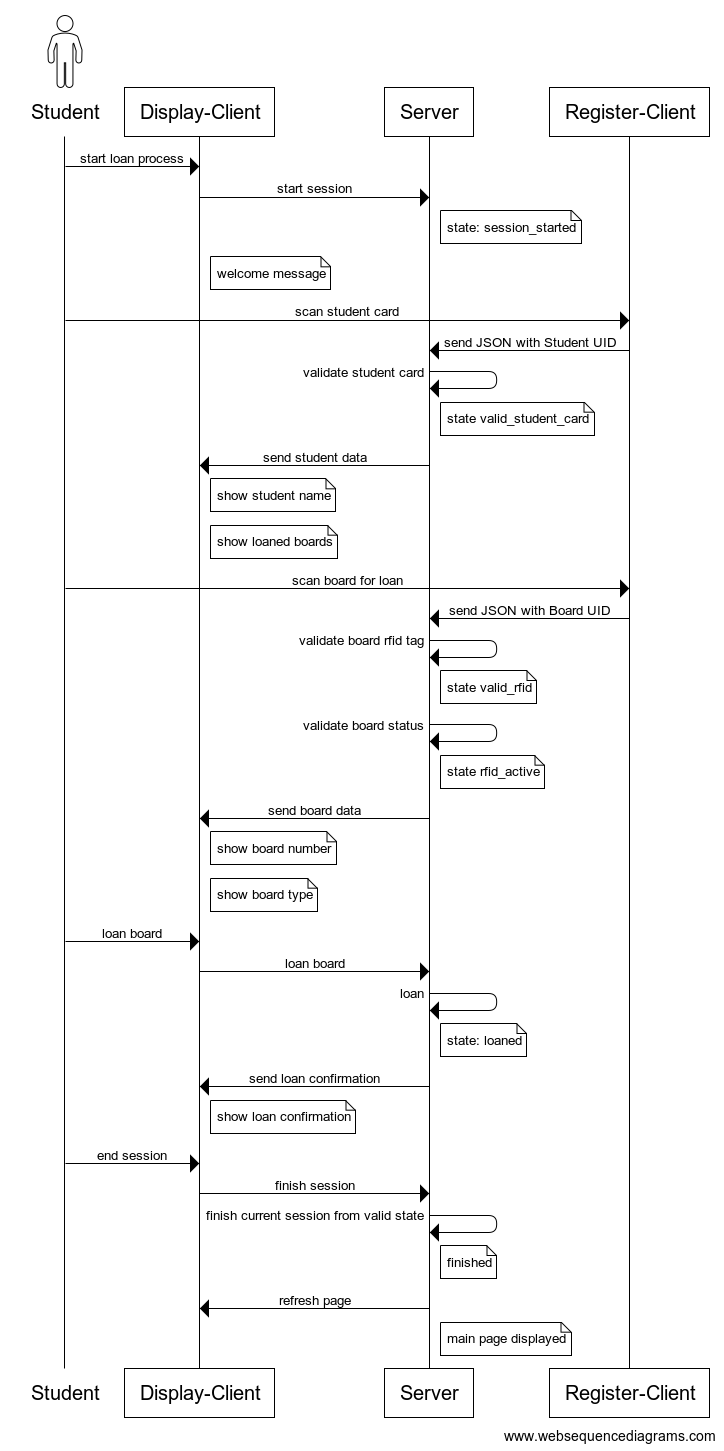
\includegraphics[width=0.8\textwidth]{gfx/seq.png}}
	\caption{UML Sequenzdiagramm der erfolgreichen Ausleihe der Lab-Loan Raspi Board}
	\label{fig:seq}
\end{figure}
Ein Sequenzdiagramm beschreibt, wie und in welcher Reihenfolge die Objekte in einem System funktionieren. In der Abschlussarbeit werden ein Sequenzdiagramm gezeigt, die auf den Abbildungen \ref{fig:seq} zu betrachten ist. Es ist ein erfolgreichen Szenario für die Ausleihe der Lab-Loan Raspi Board von einem gültigen Studierende. Das Sequenzdiagramme entspricht der oben genannte User Story \textit{"As a student, I want to loan a board so I can work at lab"}. Die meisten Kommunikation geschieht über die asynchrone Nachrichten. Zum Beispiel, es wird von Register-Klient mit dem angeschlossenen RFID-Leser nicht darauf gewartet, ob die abgelesene Studentenkarte gültig ist oder ob ein Student zum Kurs zugelassen ist. Sofort die vorherigen Ablesevorgang angeschlossen wurde und JSON-Datei dem Server geschickt, steht der RFID-Leser wieder zur Verfügung und ein RFID-Tag des Boards abgelesen werden kann. Es kann sogar sein, dass anstatt erwarteten in erfolgreichen Szenario RFID-Tags eine weitere Studentenkarte abgelesen wird (z.B. nebenstehende Kumpel der Studierende aus Spaß oder wegen der Eile lässt seine Karte ablesen vor dem Beenden des laufenden Ausleihevorgang). Obwohl es aus der Sich der Zustandsmaschine nicht zugelassen ist, eine weitere Studentenkarte zu lesen, wird trotzdem die Karte von RFID-Reader abgelesen, eine weitere JSON-Datei zum Server geschickt und weiter RFID-Leser zum nächsten Lesen freigegeben. Es ist rein die Aufgabe des Servers die ankommenden Daten zu verifizieren und den Zustandsmaschine in einem weiteren Zustand zu schalten. Die entsprechende Information mit der Begrüßung der Studierende oder Fehlermeldung wird auch vom Server generiert und dem Display-Client zum Anzeigen übergeben. Mehr über diese Vorgehensweise in entsprechenden Kapitels \ref{sec:register_client:smart}, \ref{sec:server:fsm} und \ref*{sec:display_client:js} der Implementierungsphase nachzulesen. 

\subsubsection{Endliche Zustandsmaschine mit Django FSM}
\label{sec:server:fsm:fsm}
\begin{figure}
	\centering
	\fbox{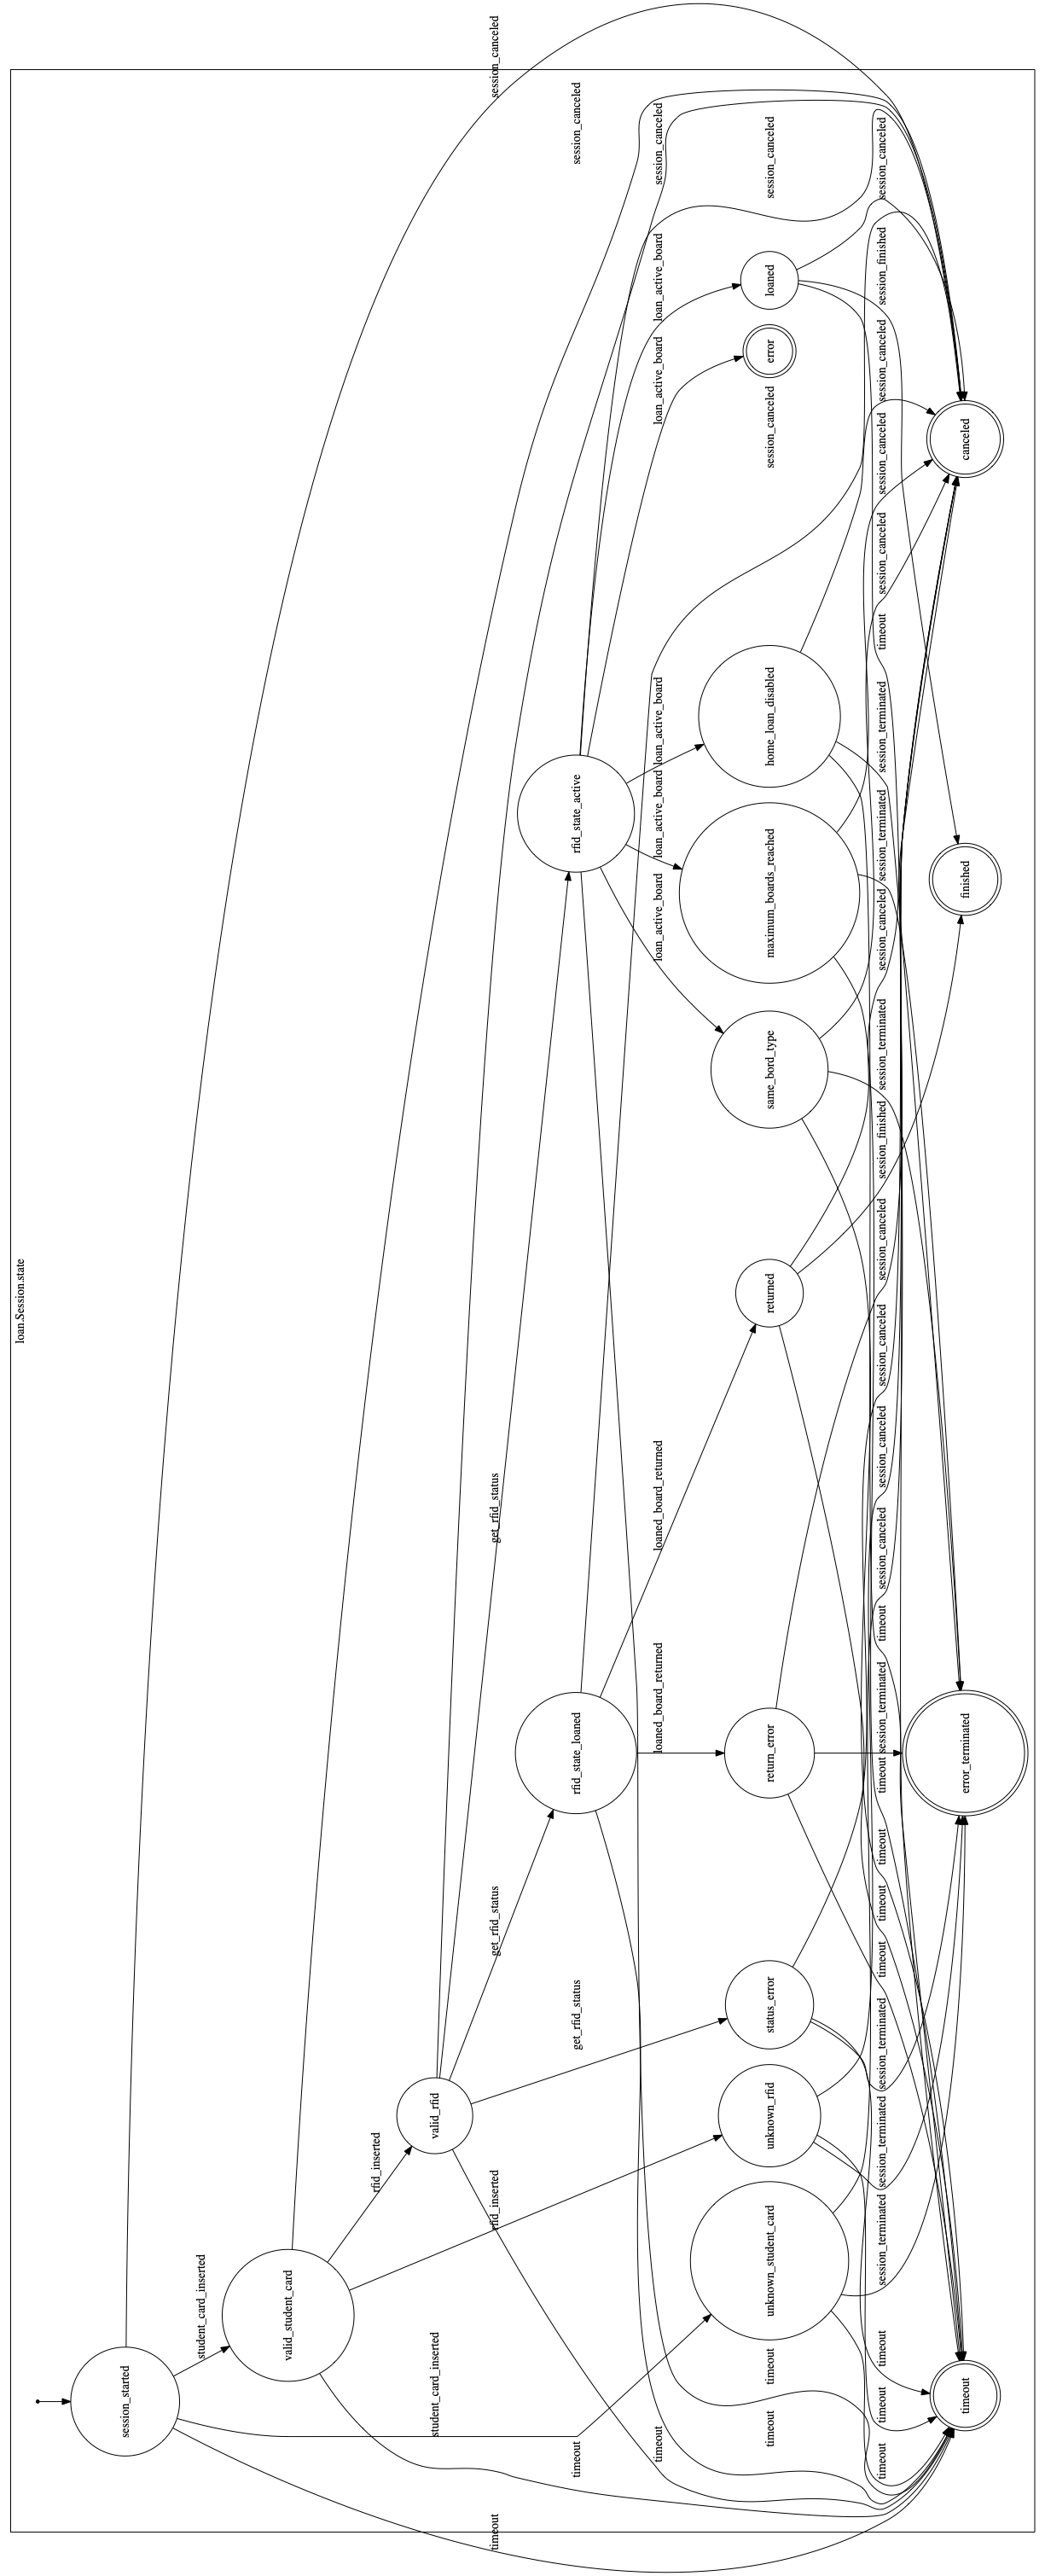
\includegraphics[width=0.7\textwidth]{gfx/transitions.png}}
	\caption{Django FSM mit Zustände und Übergänge}
	\label{fig:django_fsm_trans}
\end{figure}
Die endliche Zustandsmaschine wird mit Django FSM realisiert (auf der Abbildung \ref{fig:django_fsm_trans}). FSMField des Session Modells wird für eine automatisierte Verwaltung des Zustands der FSM verwendet. Modellmethoden werden mit dem Übergangsdekorateur markiert, sodass wird die Änderung des Zustands gemacht. Der FSM wird auf dem Zustand $session\_started"$ gestartet. Vor der Erstellung einer neuen Sitzung, wird zuerst die Felder des Modells mit der Ausführen der Funktion "clean" validiert. Falls die eine aktive Sitzung schon existiert, wird ein ValidationError ausgelöst:

\begin{lstlisting}[caption={Session clean() für die Validation des Modells},captionpos=b]
def clean(self):
	open_session = Session.objects.exclude(state__in=Session.TERMINAL_STATES).count()
	if open_session != 0:
		raise ValidationError('Active session already exists!')
	super().clean()
\end{lstlisting}

Die nächsten erlaubten bei der FSM Zustände sind: $canceled$, $timeout$, $valid\_student\_card$ und $unknown\_student\_card$. Ein Übergang in den Zustand $canceled$ is immer erlaubt und wird mit dem Drücken der "Cancel"-Taste auf einem Bildschirm des Display-Client ausgelöst. $timeout$ wird von Server behandelt und dient dazu, um zu lang gedauerte Sitzungen zwangsweise zu beenden und Display-Client für einen nächsten Versuch wieder freizumachen. Um in einem von beiden Zielzustände zu getreten, muss die Existenz der Studentenkarte in der Datenbank überprüft werden. 
\begin{lstlisting}[caption={FSM Übergang beim Ablesen der Studentenkarte},captionpos=b]
@transition(field=state, source='session_started', target=RETURN_VALUE('valid_student_card', 'unknown_student_card'))
def student_card_inserted(self, card_uid):
	try:
		card = StudentCard.objects.get(uid=card_uid)
		if card.student is not None:
			self.student_card = card
			return 'valid_student_card'
	except StudentCard.student.RelatedObjectDoesNotExist:
		return 'unknown_student_card'
	except StudentCard.DoesNotExist:
		return 'unknown_student_card'
\end{lstlisting}

Die ähnlichen Vorgänge werden bei jedem Übergang der FSM verwenden. So beispielsweise wird den Status der angelesene Board überprüft und dann wird es von FSM festgestellt, ob ein Studierende einen Board ausleihen oder zurückgeben möchte. Es wird vom Studierende nicht erfordert, die Operation zu bestimmen. 

\begin{lstlisting}[caption={FSM Übergang beim Ablesen der Board RFID-Tag},captionpos=b]
@transition(field=state, source='valid_rfid',
target=RETURN_VALUE('rfid_state_loaned', 'rfid_state_active', 'status_error'))
def get_rfid_status(self):
	board = self.get_active_board()
	if board is not None:
		if board.board_status == BoardStatus.LOANED:
			return 'rfid_state_loaned'
	elif board.board_status == BoardStatus.ACTIVE:
		return 'rfid_state_active'
	...
\end{lstlisting}

Die alle implementierte Zustände und Übergänge sind auf der Abbildung \ref{fig:django_fsm_trans} zu betrachten. Sie werden mit dem Toll $graphviz$ aus der existierenden in dem acaLoan-Projekt Modell $Session$ und seine mit dem Django FSM Zuständen und Übergange automatisiert erzeugt. Sodass werden alle Anwendungsfälle, die im Kapitel \ref{sec:design:use_cases} definiert wurden, erfolgreich mit der Verwendung der Django FSM implementiert. 

Nach jeder Änderung des Zustands wird über HTTP-Protokoll vom Server die Nachricht an Display-Client geschickt, sodass es die Änderungen dem Studierende anzeigen könnte. Die Implementierung des Clientseitiges JavaScript wird in folgenden Kapitel beschrieben.  

\section{Display-Client}
\label{sec:display_client}
Display-Client ist der dritte Bestandsteil und wird implementiert als interaktive Webseite, die einem Benutzer im in das Vollbildmodus geöffneten Webbrowser angezeigt wird. Die Client-Anwendung besteht aus zwei Teilen: 
\begin{itemize}
	\item Visuelle Darstellung eines Status einer Benutzersitzung mit in HTML beschriebenen Strukturelementen der Benutzeroberfläche mit der Verwendung eines visuelles Styling durch hinzugefügten CSS.
	\item Javascript-Code, der von einem Browser geladen und ausgeführt wird, um eine dynamische Interaktion mit dem System zu ermöglichen
\end{itemize}
Ein solcher Ansatz ermöglicht die Nutzung moderner visueller Rendering-Engines und trägt zur Erreichung der Plattformunabhängigkeit bei. 


subsection{Die Funktionsweise}
\label{sec:display_client:funkt}
Bevor der Client verwendet werden kann, muss eine spezielle URL geöffnet werden. Diese URL wird vom acaLoan-Server bereitgestellt, der liefert dem Browser sowohl eine HTML-Seite und CSS-Stylesheets zur Anzeige visueller Elemente als auch Javascript-Code zur Ausführung. Wenn der Browser die HTML-Seite lädt, werden eingehende Daten abgelesen und zusammen mit dem Rendern für einen Benutzer wird eine interne Darstellung aller auf einer Seite vorhandenen Elemente in eine baumartige Struktur namens Document Object Model. Mithilfe einer Reihe von Programmierschnittstellen, die von einem Browser bereitgestellt werden, können Attribute von DOM-Objekten oder die Struktur von DOM geändert werden. Jede Änderung am DOM, sowohl das Hinzufügen, Entfernen oder Reorganisieren von Elementen als auch das Ändern des Inhalts oder des Attributwerts des Tags, kommt sofort zur Wirkung.

Unter anderem bietet der Browser die Möglichkeit, eine asynchrone HTTP-Anforderung an einen Remote-Webserver auszuführen. In diesem Fall bedeutet asynchron, dass die Benutzerinteraktion mit der Webseite für die Zeit, in der die Anforderung ausgeführt wird, nicht blockiert wird. Die Standard-API-Schnittstelle für solche Vorgänge heißt XMLHttpRequest. Diese Programmierschnittstellen werden vom Browser über eine Javascript-Codeausführung verfügbar gemacht. Der Entwickler kann ein Javascript-Programm erstellen, das mit externen Diensten kommunizieren und  DOM-Elemente aktualisieren darf, um Änderungen anzuzeigen.

Die Kombination dieser Funktionen dient als Grundlage für die Erstellung eines interaktiven Client-Flows:
\begin{enumerate}
	\item Die Clientanwendung stellt eine Kommunikation mit einem Server her und empfängt Aktualisierungen über den aktuellen Status einer Benutzerinteraktion
	\item Wenn der Server mit dem aktuellen Status antwortet, kann er mit einem derzeit bekannten Anwendungsstatus eines Clients verglichen werden, und bei Bedarf können Änderungen am DOM vorgenommen werden.
	\item Da HTTP-Anforderungen für einen Benutzer transparent sind und Änderungen am DOM sofort sichtbar sind, entsteht eine echte interaktive Erfahrung.
\end{enumerate}

\subsection{Start Webseite des acaLoan-Projekts}
\label{sec:display_client:start}
\begin{figure}[h!]
	\centering
	\fbox{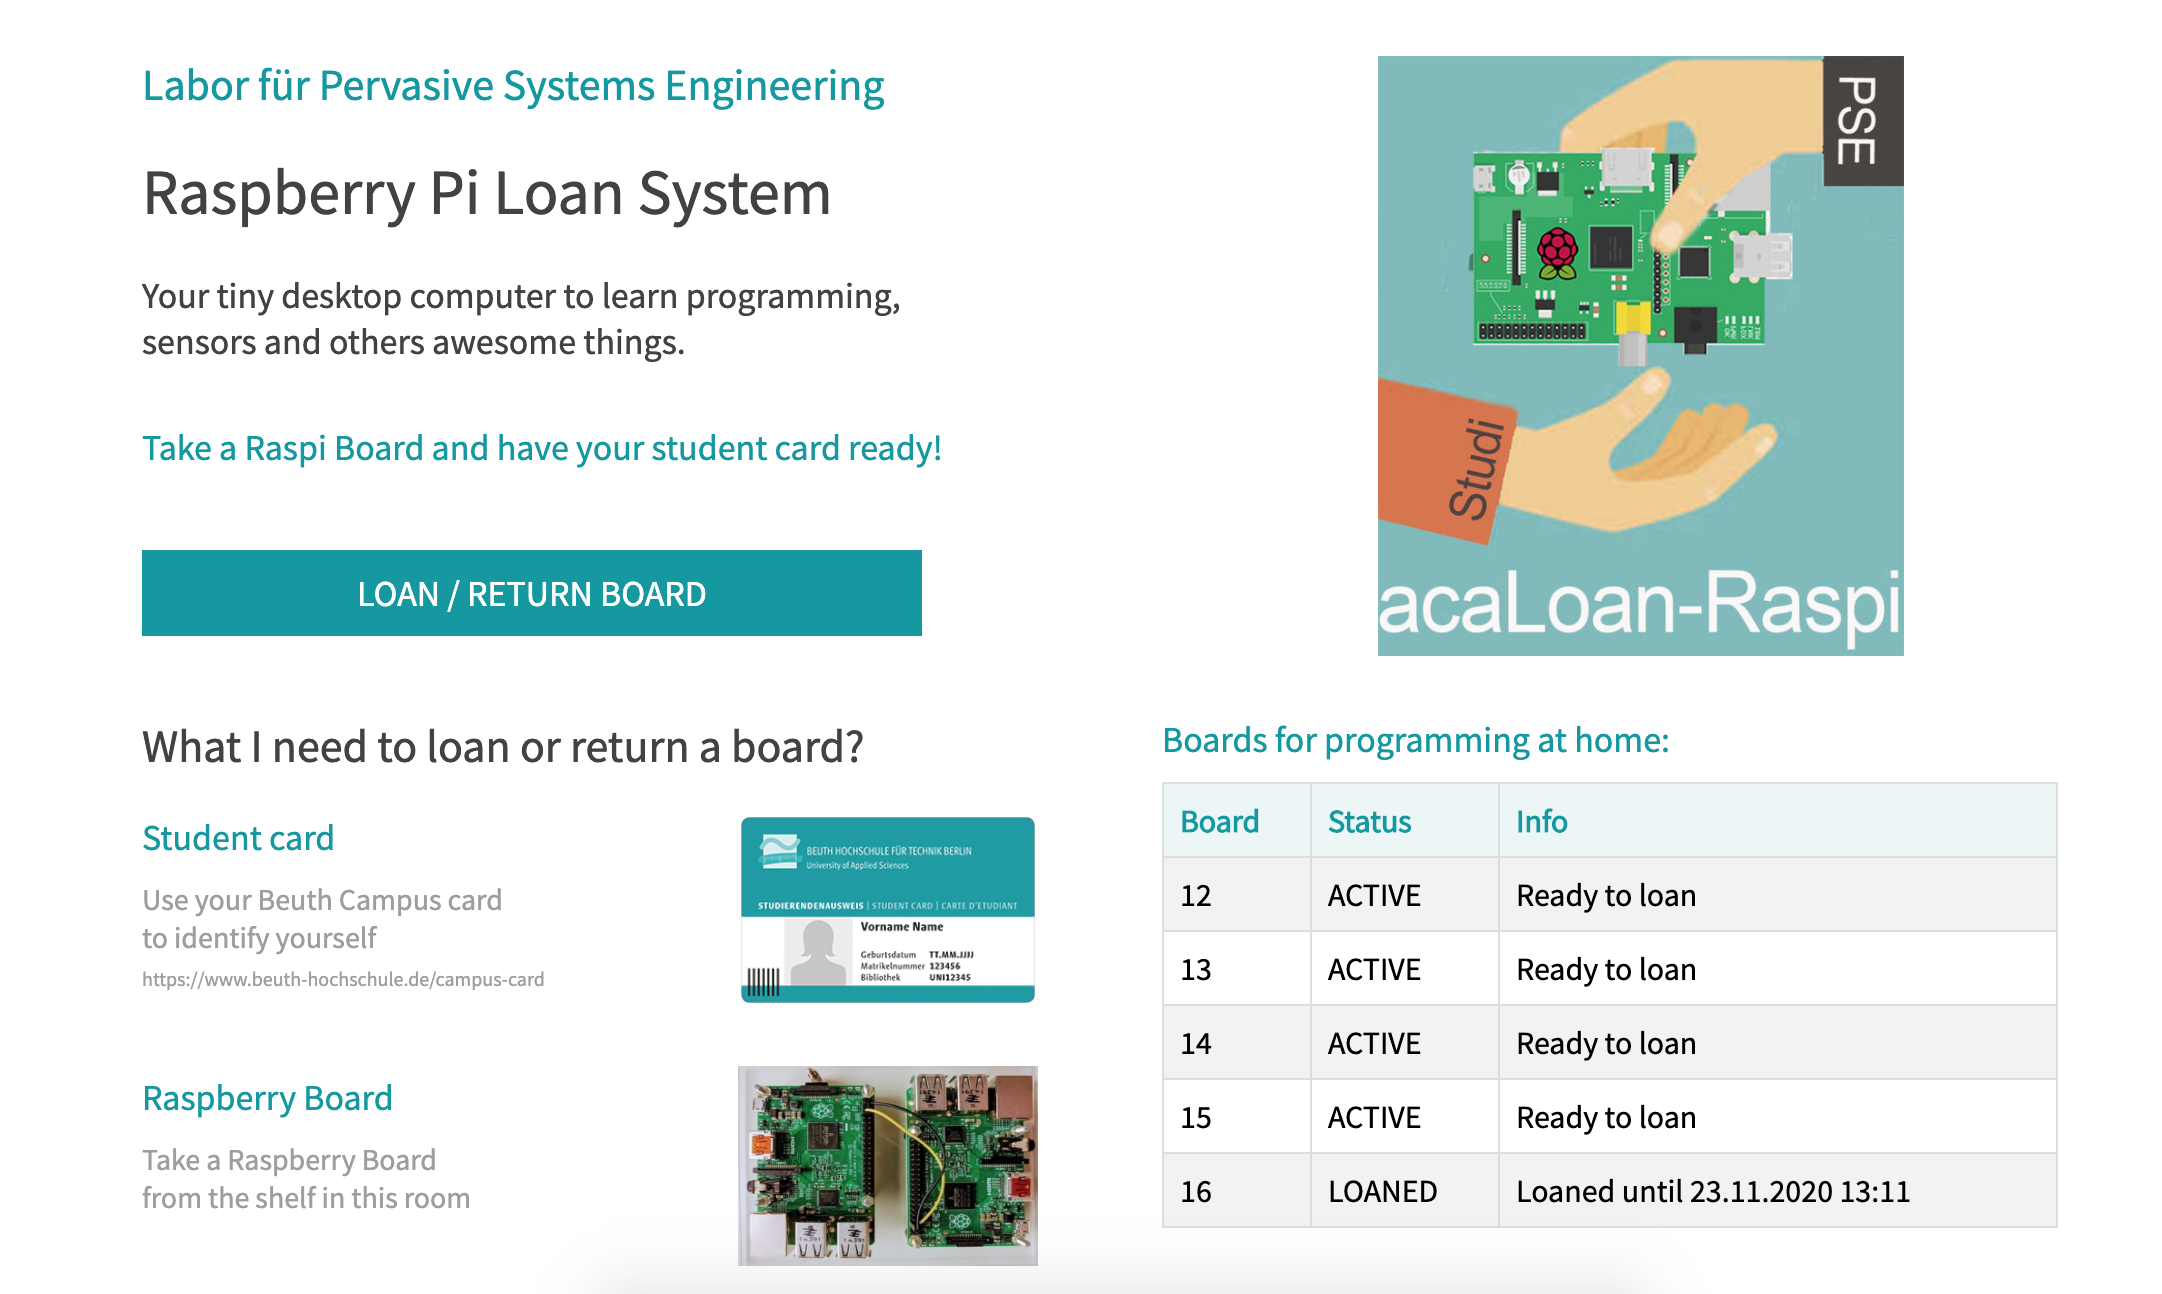
\includegraphics[width=1\textwidth]{gfx/start.png}}
	\caption{Start Webseite des acaLoan-Projekts}
	\label{fig:start_page}
\end{figure}
Zunächst wird dem Benutzer eine Zielseite angezeigt. Diese Seite verfügt über eine HTML-Taste (siehe Abbildung \ref{fig:start_page}), die der Studierende drucken muss, um eine neue Benutzersitzung anzufangen. Durch Klicken auf diese Taste "Loan / Return Board" wird eine synchrone HTTP-POST-Anforderung an einen Server gesendet, der die Erstellung einer neuen interaktive Benutzersitzung anfordert. Im Fehlerfall antwortet der Server mit einem Fehler-HTTP-Statuscode und der Browser zeigt eine Fehlermeldung an.
\begin{lstlisting}[caption={[Fehler-HTTP-Statuscode] },captionpos=b]
Forbidden: /loan/api/sessions
"POST /loan/api/sessions HTTP/1.1" 403 47
\end{lstlisting}
Wenn keine aktive Sitzung vorhanden ist, treten folgende Ereignisse auf:
\begin{enumerate}
	\item Der Server erstellt eine neue Benutzersitzung
	\begin{lstlisting}[caption={[HTTP-Statuscodes für die neue Sitzung] },captionpos=b]
	"GET /loan/start HTTP/1.1" 200 5423
	"POST /loan/api/sessions HTTP/1.1" 201 120
	"GET /loan/api/sessions/17 HTTP/1.1" 201 216
	\end{lstlisting}
\item Der Server antwortet mit dem HTTP-Statuscode 201 und liefert dem Browser das grundlegende Layout der Sitzungsinteraktionsseite. In der Beispiel oben wurden die neue Benutzersitzung mit der Nummer 17 erstellt.
\item Der Browser verarbeitet die HTML-Seite und lädt zusätzliche statische Elemente wie CSS-Stylesheets und JavaScript-Code vom Server.
\item Die HTML-Seite wird generiert, JS-Code wird ausgeführt. Die interaktive Sitzung hat begonnen. Die ist auf der Abbildung \ref{fig:web01} angezeigt. In dem Zustand der FSM $session\_started$ wird zuerst keine Information gegeben, wer der Studierende ist und mit welchem Board gearbeitet ist. Die Webseite zeigt dem Studierende nur die Hinweise, die ihn das Prozess der Ausleihe-/Rückgabe erleuchten können. 
\begin{figure}[h!]
	\centering
	\fbox{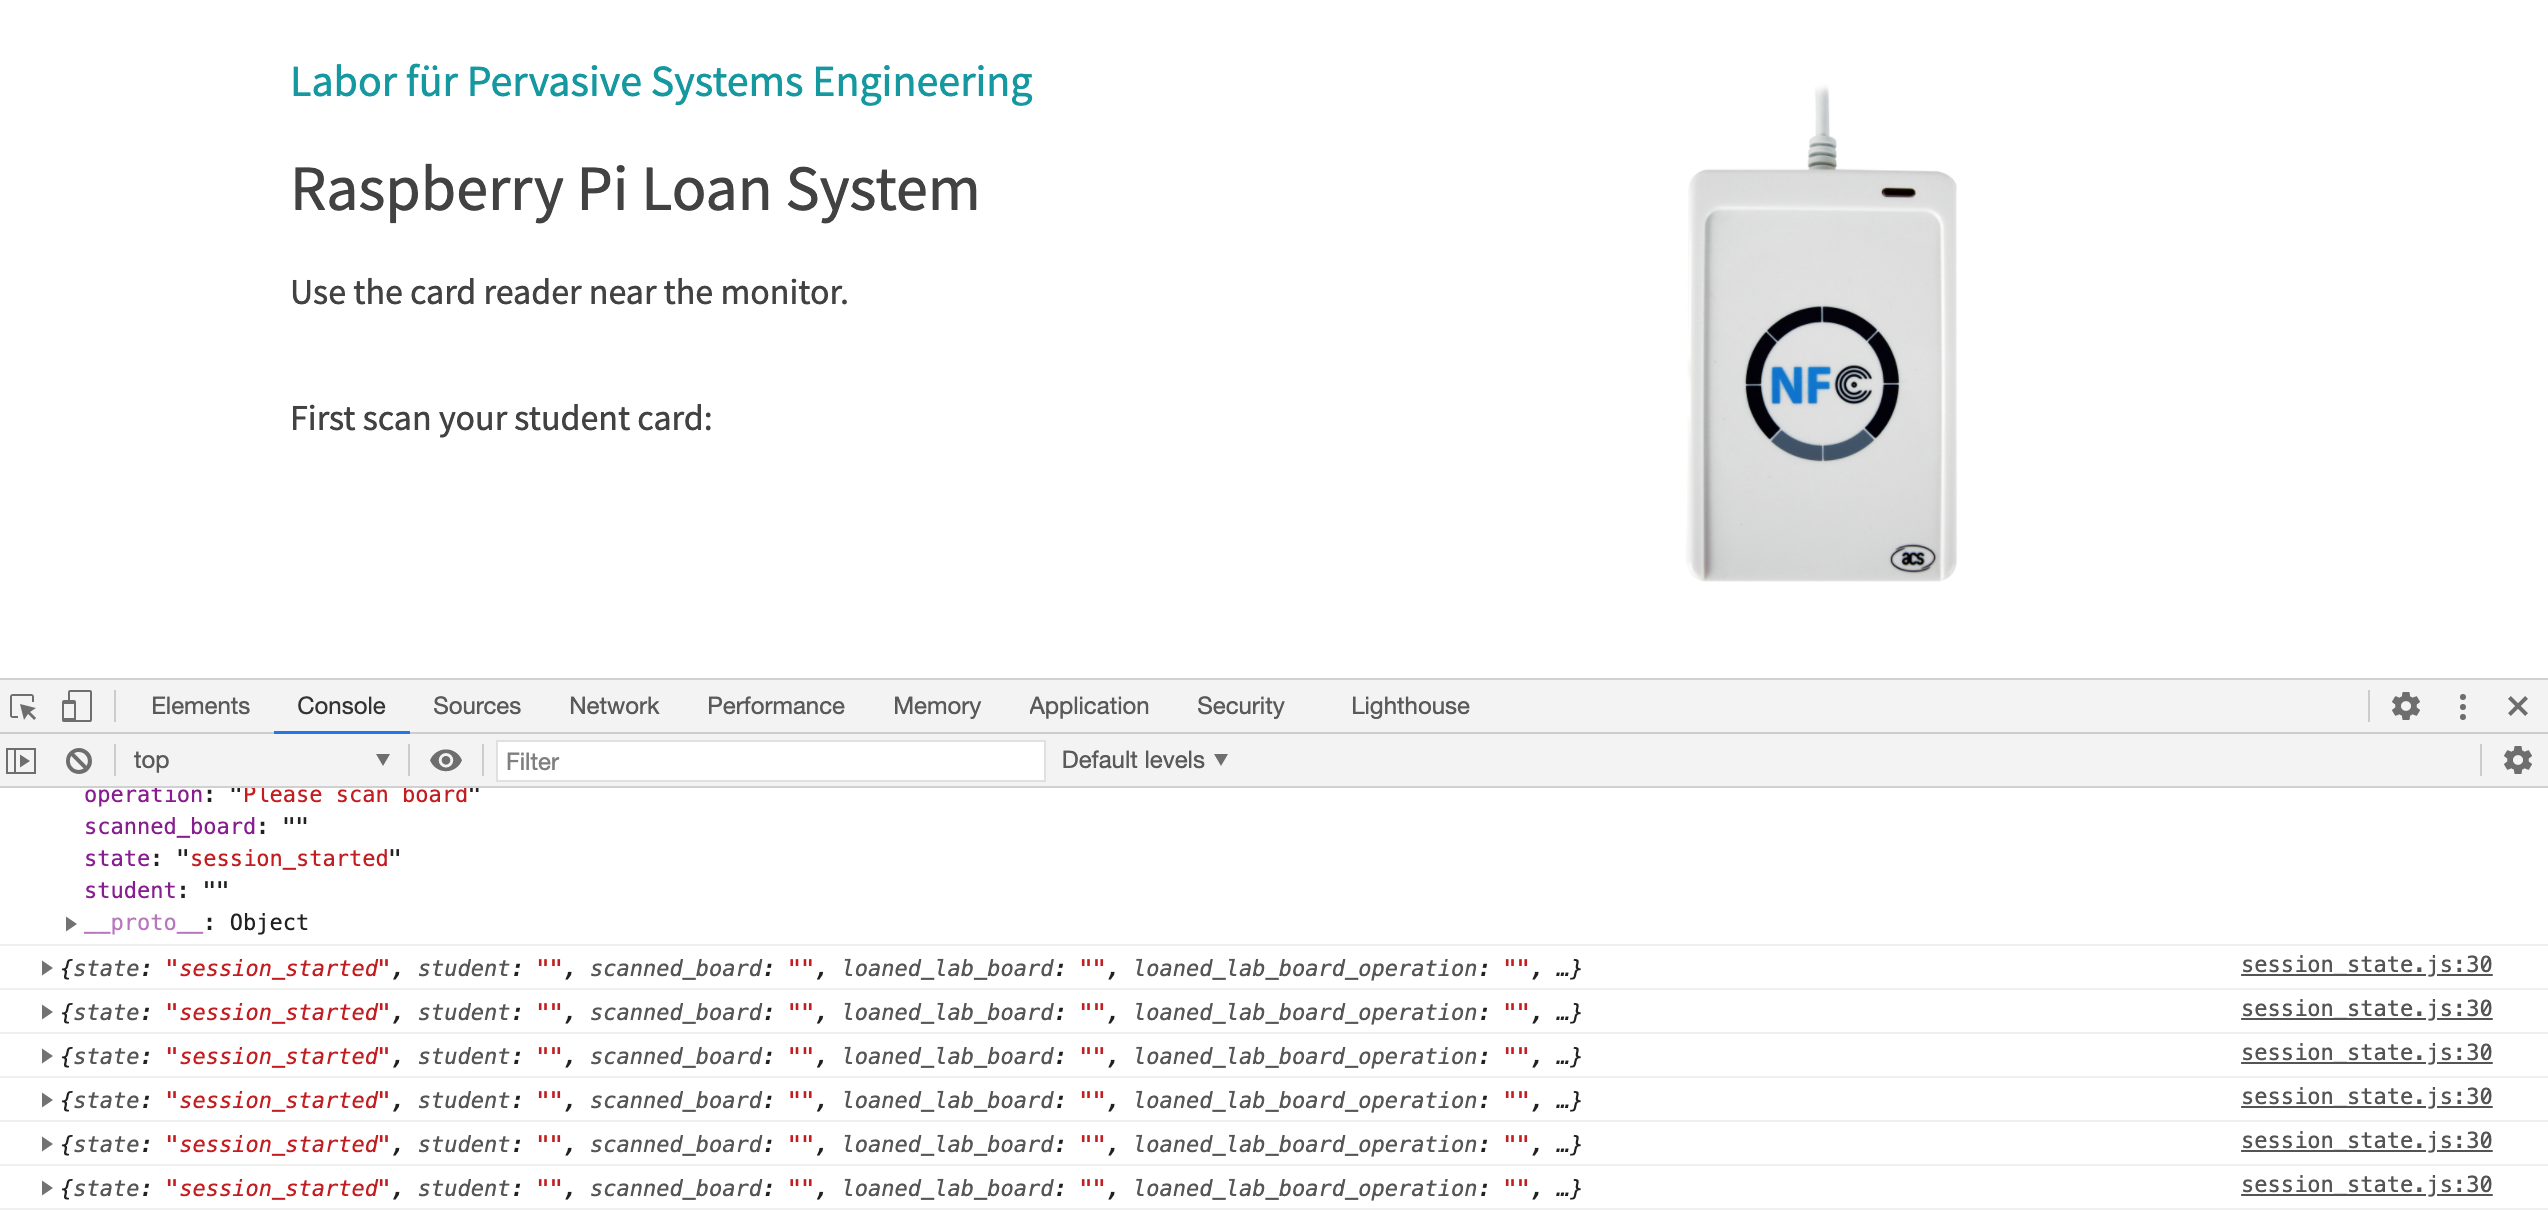
\includegraphics[width=1\textwidth]{gfx/web01.png}}
	\caption{Webseite für eine neue Benutzersitzung mit dem Console-Log}
	\label{fig:web01}
\end{figure}
\end{enumerate}

\subsection{Interaktive Benutzersitzung mit JavaScript}
\label{sec:display_client:session}
Nachdem die Benutzersitzung gestartet ist. dient die folgenden Bedingungen:
\begin{itemize}
	\item Der Sitzungsstatus wird auf dem Server geändert
	\item Der Benutzer interagiert mit einem Elemente der angezeigten Webseite
\end{itemize}
Da das HTTP-Protokoll keine bidirektionale Kommunikation bietet und die Möglichkeiten des Servers, Daten proaktiv an einen Client zu übertragen, sehr begrenzt sind, muss regelmäßig nach einer Änderung des Sitzungsstatus gefragt werden. Um dies zu erreichen, legt der Javascript-Code eine regelmäßige Aktualisierung des Sitzungsstatus fest durch Registrieren eines Timer-Ereignisses mit dem Aufrufen einer setInterval() -Funktion. 
\begin{lstlisting}[caption={function session\_started()},captionpos=b]
function session_started(body) {
	console.log("Started session with id " + body.id)
	active_session_id = body.id
	session_refresh_timer = setInterval(refresh_session_state, 1000)}
\end{lstlisting}
Die Entwicklung mit einfachen Javascript-APIs ist umständlich und fehleranfällig. Um die Codebasis zu vereinfachen und später zu machen Unterstützung und Änderungen einfacher, eine Reihe von Frameworks wurden erstellt. Ziel eines solchen Frameworks ist es, Entwickler von zu isolieren
interne Komplexität von reinen JS-APIs und bieten browserübergreifende Kompatibilität, wenn verschiedene Browser implementiert werden bestimmte API auf andere Weise. Dieses Projekt wurde mit einer plattformübergreifenden Javascript-Bibliothek namens jQuery erstellt. In Quellcode unten wird mit $jQuery.ajax( url [, settings ] )$ eine asynchrone HTTP-Anforderung (Ajax) ausgeführt. 
\begin{lstlisting}[caption={Function refresh\_session\_state()},captionpos=b]
function refresh_session_state() {
	$.ajax({url: "api/sessions/"+active_session_id, method: "GET"})
	.done(handle_session_event)
	.fail(function() {
		clearInterval(session_refresh_timer)
		alert("Timeout/Canceled. Please start again!")
		window.location.replace("/loan")
		})}
\end{lstlisting}

Die Funktion $handle\_session\_event$ wird nach erfolgreichem Abschluss einer Ajax-Anforderung ausgerufen und hat die folgenden Funktionsweise:
\begin{itemize}
	\item Die Funktion verwendet die XMLHttpRequest() nach Browser-API, um eine asynchrone HTTP-Anforderung an den Server zu senden
	\item Die asynchrone HTTP-Anforderung wird so eingerichtet, dass eine vom Benutzer bereitgestellte Funktion aufgerufen wird, wenn der Server eine erfolgreiche Antwort liefert.
	\item Basierend auf dem Inhalt der Antwort wird der Status des DOM angepasst, um den Sitzungsstatus widerzuspiegeln und den Benutzer über die erforderlichen Aktionen zu informieren. Die Fehlermeldungen werden auch von dieser Funktion über Status des DOM angepasst, z.B. in folgenden Quellcode wird es die Fehlermeldung gegeben über Verbot einen Board nach Hause auszuleihen:
	\begin{lstlisting}[caption={Änderung des DOM im Fall des Verbot der Home-Ausleihe},captionpos=b]
	if (body.state == "home_loan_disabled") {
		$("#student_name").text("You can not loan board to work a home")
		$("#operation_info").text("Home loan is disabled. Ask teaching assistant or administrator for a help")
		$("#warning_picture").show()
		decorate_terminate_state(body)}
	\end{lstlisting}
	\item Der neue Sitzungsstatus wird im Client zur späteren Bezugnahme gespeichert.
\end{itemize}

\subsection{Client-Server-Kommunikationsprotokoll}
\label{sec:display_client:protokoll}
Beim regelmäßigen Abrufen von Sitzungsaktualisierungen vom Server erwartet der Client, dass der Server mit JSON-Nachrichten antwortet. Die Clientanwendung analysiert diese Nachrichten und vergleicht sie mit dem vorherigen bekannten Status. Hier wird es auch auf die UIDs der Studentenkarten und RFID-Tags der Rapsi-Boards erwartet. 
\begin{lstlisting}[caption={Sitzungsaktualisierungen mit JSON},captionpos=b]
if input_type not in ["card", "tag", "cancel_button", "terminate_button", "get_rfid_status", "return_scanned_board_button", "loan_scanned_board_button", "finish_button"]:
	return HttpResponseBadRequest()
...
elif input_type == "cancel_button":
	session.session_canceled()
elif input_type == "finish_button":
	session.session_finished()
elif input_type == "get_rfid_status":
	session.get_rfid_status()
elif input_type == "return_scanned_board_button":
	session.loaned_board_returned()
elif input_type == "loan_scanned_board_button":
	session.loan_active_board()
elif input_type == "terminate_button":
	session.session_terminated()
\end{lstlisting}
Einem Client bekannten Status der endliche Zustandsmaschine wird dem im Kapitel \ref{sec:design:fsm} und \ref{sec:server:fsm:fsm} beschriebenen Sitzungsstatus zugeordnet. Beispielweise in dem Anwendungsfall "Ausleihe des Home-Loan Boards" (Kapitel \ref{sec:design:use_cases:home_loan}) gibt es einen Übergang aus dem Zustand $rfid\_state\_active$ nach entweder erfolgreichem Zustand $loaned$ oder enem von mehreren vordefinierten fehlerhaften Zustände. 

\begin{lstlisting}[caption={Übergang aus dem Zustand rfid\_state\_active},captionpos=b]
@transition(field=state, source='rfid_state_active', target=RETURN_VALUE('loaned', 'home_loan_disabled', 'error', 'maximum_boards_reached', 'same_bord_type'))
def loan_active_board(self):
	result = self.board_loaned()
	if result == 'loaned':
		Board.loan_board(self.raspi_tag)
return result
\end{lstlisting}

Während des Beispielübergangs der FSM mithilfe der Funktion $board\_loaned$ wird der aktive Studierende aus der Sitzung mit dem Aufruf der Funktion $get\_active\_student$ abgerufen, um seine Rechte zum Home-Ausleihe zu überprüfen und eine Liste der zugewiesenen ihm Boards zu bekommen. Nachdem wird es festgestellt, dass der Studierende den Board ausleihen darf, wird die neue Aktion in Datenbank erstellt.

\begin{lstlisting}[caption={Neue Aktion in der Datenbank während des FSM Übergangs},captionpos=b]
def loan_board_action(student, board, operation, timestamp=datetime.datetime.now):
	loaned_board_action = Action(student=student, board=board, operation=operation)
	loaned_board_action.save()
\end{lstlisting}
\begin{figure}[hb!]
	\centering
	\fbox{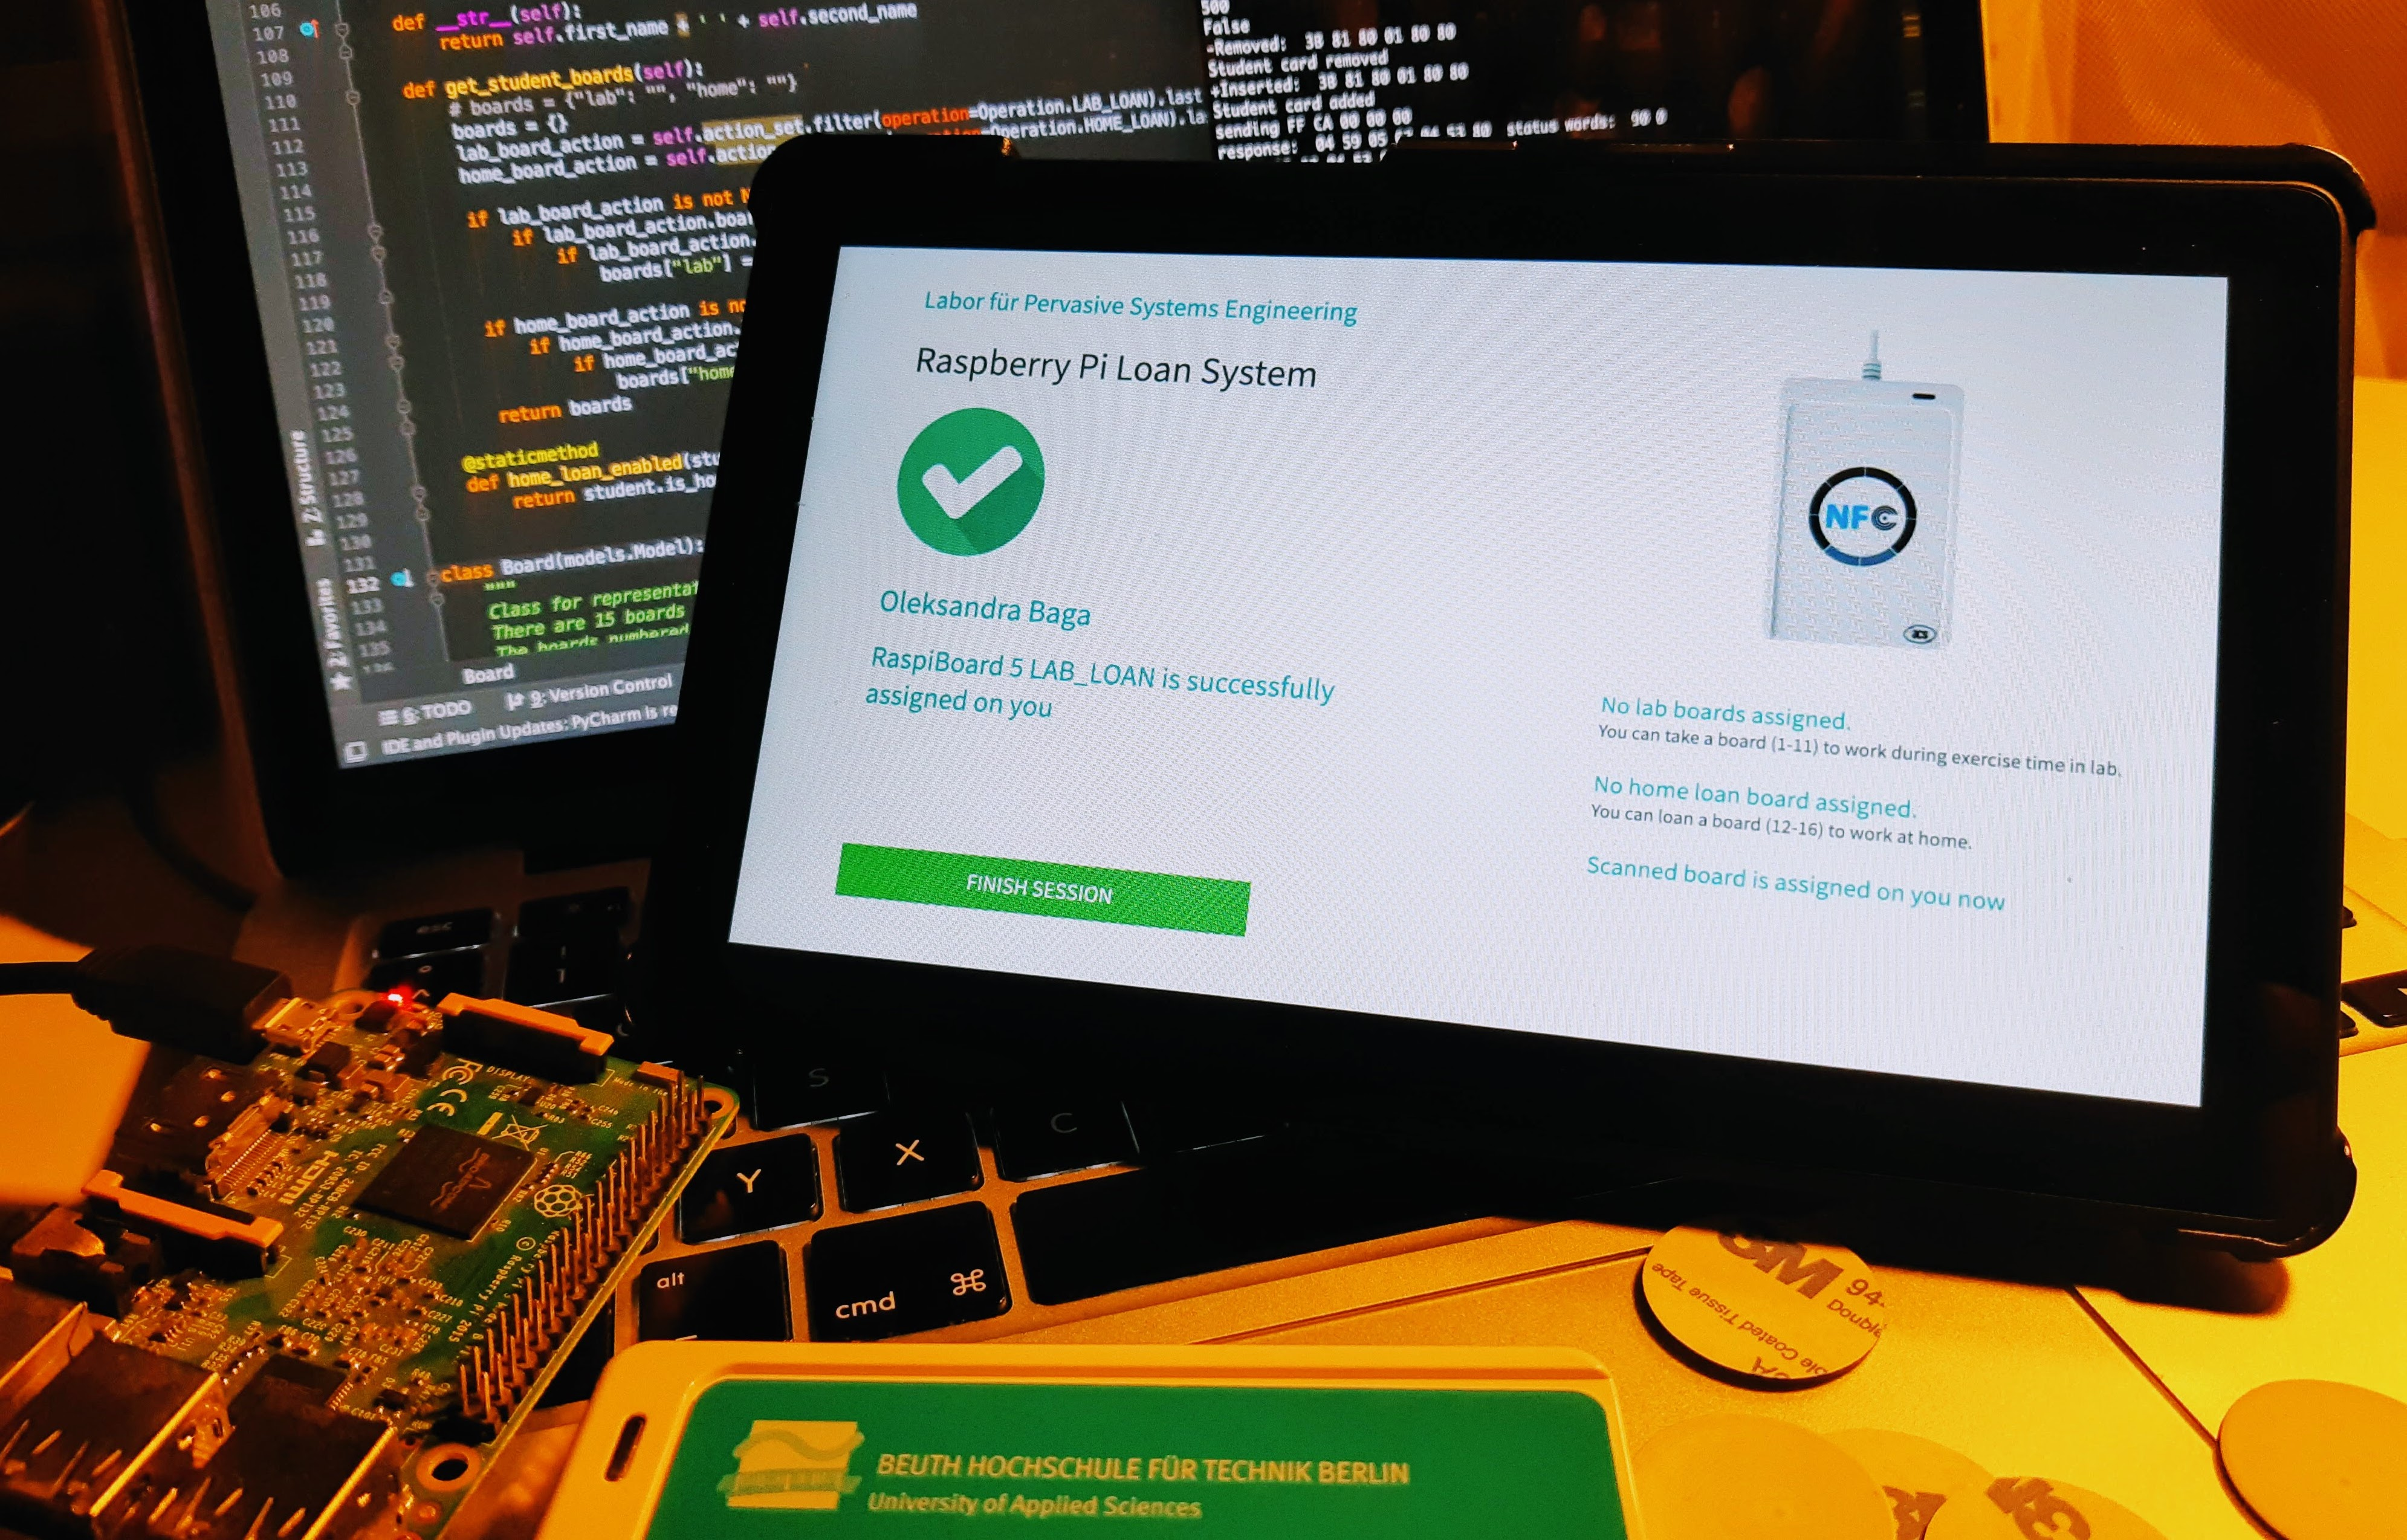
\includegraphics[width=1\textwidth]{gfx/fsm_end.jpg}}
	\caption{Webseite für einen Endzustand nach der Ausleihe des Boards}
	\label{fig:fsmend}
\end{figure} 
Operation wird während des Ausführen der Funktion abhängig vom dem Typ des Boards bestimmt und kann entweder $Operation.HOME\_LOAN$ für den Board $BoardType.HOME\_LOAN$ oder $Operation.HOME\_LOAN$ für den Board $BoardType.HOME\_LOAN$ sein. Endlich wird der Status des Boards auf "Loaned" gesetzt. 
\begin{lstlisting}[caption={Wechseln des Statuses des Boards von active zu loaned},captionpos=b]
def loan_board(raspi_tag):
	# Update the status of the board with raspi_tag
	Board.objects.filter(raspi_tag=raspi_tag).update(board_status=BoardStatus.LOANED)
\end{lstlisting}

Die endliche Zustandsmaschine in einen Zustand $loaned$ gewechselt. Dann wird es mit der nächsten regelmäßigen Abrufen von Sitzungsaktualisierungen wieder den Status der DOM angepasst, um eine erfolgreiche finale Zustand zu stylen. So werden mittels JavaScript die Tasten "Loan Board" und "Cancel" Tasten verborgen und die neue Taste "Finish" angezeigt, beim deren Drucken wird FSM in einem Endzustand gewechselt. Somit wird der Benutzersitzung beendet, da der Zustand "finished" ein von mehreren Endzustände ist, mit denen FSM beenden darf und somit die neue Sitzung angefangen werden darf. Den Display-Client mit einer Webseite nach dem erfolgreichen Ausleihe eines Boards ist auf der Abbildung \ref{fig:fsmend} gezeigt.

\section{Automatisierten Tests}
\label{sec:testing}
Django bietet ein Testframework mit einer kleinen Hierarchie von Klassen, die auf der unittest-Python-Standardbibliothek aufbauen. Trotz des Namens eignet sich dieses Testframework sowohl für Unit- als auch für Integrationstests. Das Django-Framework fügt API-Methoden und -Tools hinzu, mit denen das Web- und Django-spezifische Verhalten getestet werden kann. Mit diesen können Sie Anforderungen simulieren, Testdaten einfügen und die Ausgabe Ihrer Anwendung überprüfen \cite{website:djangoTest}.

Für Testing muss eine Datenbank mit Datensätzen gefühlt werden. In dem Fall des acaLoan-Project bedeuted es, sowohl notwendige UIDs der Studentenkarten als auch die Namen, Vornamen und sogar Matrikelnummern sollen bei jedem Testen erzeugt werden. Das gilt auch für die UIDs des Boards mit den verschiedenen Status und Typen. Alle Zustände die endliche Zustandsmaschine sollen auch getestet werden, dafür muss nicht nur FSM in einem Zustand gesetzt wird sondern auch die notwendigen Datensätze in der Tabelle "Aktion" und "Session" vorbereiter werden. Jedes Mal es manuell wiederholen wäre zu aufwändig. Deshalb wirden die $factory\_boy-Bibliothek$ (nach dem Vorbild von Factory Girl in Rails) benutzt, um die Daten für Tests zu generieren. In Django wurden Daten für Tests als Fixtures bezeichnet, die aus Dateien im Code geladen wurden. Beispielweise in dem Quellcode wird so viel wie notwendig "korrekten" UID generiert (sie sind nur aus der Datensicht korrekt, da sie nicht von offiziellen Herstellen gegeben wurden und sind somit nicht einzigartig)

\begin{lstlisting}[caption={Factory für UIDs},captionpos=b]
class FuzzyUid(factory.fuzzy.BaseFuzzyAttribute):
	def __init__(self, length):
		self.length = length
		super().__init__()
		
	def _segment(self):
		x = randgen.randint(0, 255)
		return "{:02X}".format(x)
	
	def fuzz(self):
		return ' '.join([self._segment() for _ in range(self.length)])
\end{lstlisting}

Da eine Studentenkarte muss aus 7 Segmenten bestehen und ein RFID-Tag aus nur 4 Segmenten, ist der Rest der Struktur gleich und die FuzzyUid-Klass kann für die Generierung sowohl UIDs der Studentenkarten als auch RFID-Tags verwendet werden: es wird nur den Parameter $lenght$ angepasst.

\begin{lstlisting}[caption={StudentCardFactory},captionpos=b]
class StudentCardFactory(DjangoModelFactory):
	class Meta:
		model = StudentCard
	atr_hex = ATRCardType.STUDENT_CARD_ATR
	uid = FuzzyUid(length=7)  
\end{lstlisting}
$Factory\_boy$ verwendet $Fake\-Factory (Faker)$, um zufällige Werte zu generieren. Das ist besonders nützlich für die Generierung von Namen, Vornamen, Adressen, IP4-Adressen und andren Sätzen, die in realen Datenbanken verwendet werden können. Benutzung der $Locale de\_DE$ zulässt die deutschen Namen und Städten zu generieren. Im Beispiel unten werden "die Studierende" generiert, für denen die Matrikelnummern und HRZ-Nummern werden als zufälligen Werten in Rahmen vordefinierten Bereich ausgewählt.   
\begin{lstlisting}[caption={StudentFactory},captionpos=b]
class StudentFactory(DjangoModelFactory):
	class Meta:
		model = Student
	student_card = factory.SubFactory(StudentCardFactory)
	first_name = factory.Faker('first_name')
	second_name = factory.Faker('last_name')
	matricul_no = factory.Faker('random_int', min=850000, max=950000)
	hrz_no = factory.Faker('random_int', min=65000, max=69000)
	group = StudentGroup.A_GROUP
	is_home_loan_enabled = True
\end{lstlisting}

Während der mehreren Ausführungen der Tests es hat sich ein paar Mal Fehler aufgetreten: von Factory mehr als ein Student mit der gleichen Matrikelnummer generiert wurde. In Django Model "Student" ist das Feld $matricul\_no$ mit $unique=True$ markiert. Die Tests müssen einfach erneut geladen werden, dann tritt höchstwahrscheinlich der Fehler nicht wieder auf. 

Der Django-Test ist eine Funktion, die mit einem vorbereiteten Inhalt die Änderungen in der Datenbank macht und dann vergleicht das Ergebnis mit einem erwarteten Zustand. Sodass prüft folgende Funktion, ob einem Studierende, der von Factory erzeugt wurde und dem den Flag $home\_loan\_enabled$ nicht gesetzt wurde, eine Home-Ausleihe gelingen kann: 
\begin{lstlisting}[caption={Test für einen Student},captionpos=b]
def test_home_loan_disabled(self):
	session = Session.objects.create(state='rfid_state_active', student_card=self.student_home_disabled.student_card,
	raspi_tag=self.home_board_active.raspi_tag)
	self.assertEqual(session.board_loaned(), 'home_loan_disabled')
\end{lstlisting}

\begin{figure}[h!]
	\centering
	\fbox{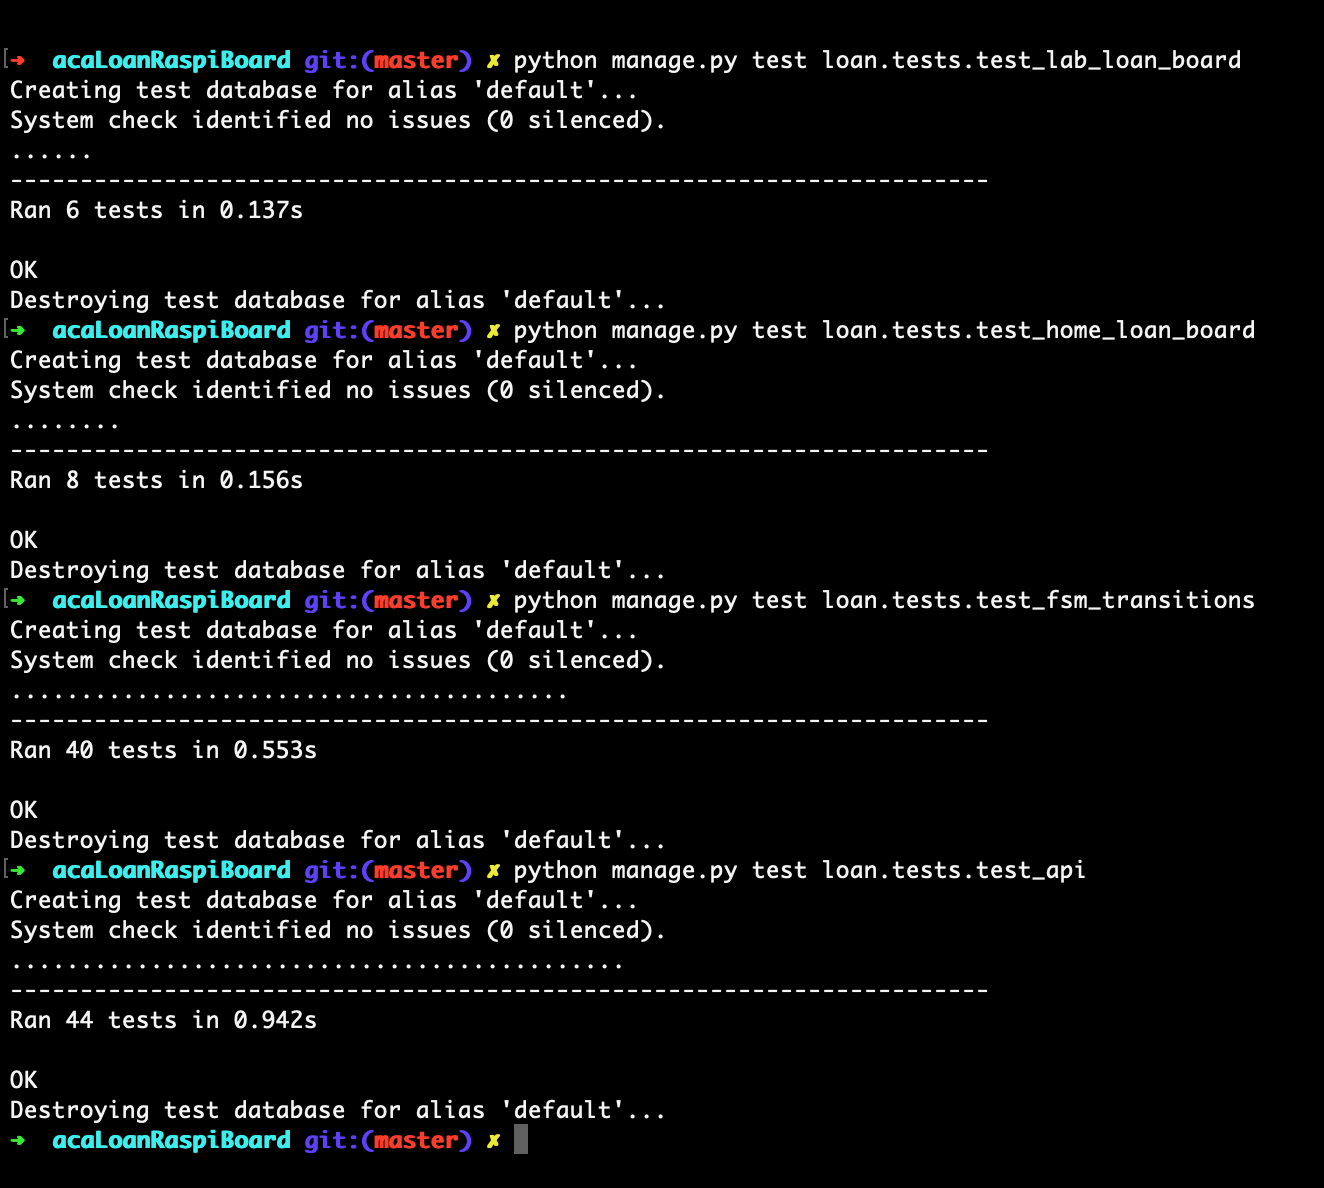
\includegraphics[width=0.8\textwidth]{gfx/test.png}}
	\caption{Terminal nach der Ausführung aller Tests}
	\label{fig:test}
\end{figure}

Sodass wurde die REST API, die endliche Zustandsmaschine und alle Anwendungsfälle des acaLoan-Systems fehlerfrei getestet. Insgesamt 98 Testfunktionen wurden geschrieben und ausgeführt. 